\documentclass[11pt]{article}

\usepackage[a4paper,margin=25mm,headheight=14pt]{geometry}
\usepackage[T1]{fontenc}
\usepackage[utf8]{inputenc}
\usepackage{libertinus}
\usepackage{microtype}
\usepackage{amsmath,amssymb,amsthm,mathtools,bm,mathrsfs}
\usepackage{booktabs,longtable,tabularx,array}
\usepackage{graphicx}
\usepackage{enumitem}
\usepackage{xcolor}
\usepackage{hyperref}
\usepackage[nameinlink,capitalise,noabbrev]{cleveref}
\usepackage{fancyhdr}
\usepackage{listings}
\usepackage{caption}
\usepackage{subcaption}
\usepackage{url}
\usepackage{needspace}
\allowdisplaybreaks

\hypersetup{
  pdftitle={Holonomic Rank, Exact Overlaps, and Non-P-Recursiveness in the Fabius--Rvachev System},
  pdfauthor={Prepared for Vladimir Reshetnikov},
  pdfsubject={Finite sinc-product ODEs, signed-overlap entropy, Thue--Morse spectra, and infinite-rank limits},
  pdfkeywords={Fabius function, Rvachev up function, Thue--Morse, D-finite, P-recursive, Bernoulli convolution, q-analog, Bell polynomial, Bernoulli polynomial},
  colorlinks=true,
  linkcolor=blue!48!black,
  citecolor=green!35!black,
  urlcolor=blue!55!black
}

\pagestyle{fancy}
\fancyhf{}
\fancyhead[L]{Holonomic frontiers of the Fabius--Rvachev system}
\fancyhead[R]{\thepage}
% Canonical project-wide mathematical notation.
% Canonical mathematical notation for active FabiusFunction LaTeX documents.
%
% This file is intentionally a plain TeX input rather than a LaTeX package.
% Every standalone document loads it by an explicit path relative to that
% document's directory; included fragments inherit the definitions from their
% root document.  Keep this file independent of document layout and metadata.
%
% Contract:
%   * one command has one mathematical meaning throughout the active corpus;
%   * names encode semantic roles rather than a document-local choice of letter;
%   * visually similar but differently normalized objects have different print;
%   * every command below is defined normatively in the notation catalogue.
%
% The active corpus excludes docs/archive/.  Historical sources may retain
% their original notation only inside an explicitly labelled quotation.

\makeatletter
\@ifundefined{mathbb}{%
  \PackageError{fabius-notation}{The amssymb package must be loaded first}%
    {Load amsmath and amssymb before inputting fabius-notation.tex.}%
}{}
\@ifundefined{operatorname}{%
  \PackageError{fabius-notation}{The amsmath package must be loaded first}%
    {Load amsmath before inputting fabius-notation.tex.}%
}{}
\makeatother

% Version stamp used by the catalogue and by static audits.
\newcommand{\FabiusNotationVersion}{2026-08-31}

% Number systems.  NaturalNumbers is explicitly the nonnegative convention.
\newcommand{\NaturalNumbers}{\mathbb{N}_{0}}
\newcommand{\PositiveIntegers}{\mathbb{N}_{>0}}
\newcommand{\IntegerNumbers}{\mathbb{Z}}
\newcommand{\RationalNumbers}{\mathbb{Q}}
\newcommand{\RealNumbers}{\mathbb{R}}
\newcommand{\ComplexNumbers}{\mathbb{C}}
\newcommand{\ExtendedRealNumbers}{\overline{\mathbb{R}}}

% The three principal Fabius--Rvachev functions.  Subscripts are deliberate:
% a bare F and a calligraphic F have several unrelated uses in the corpus.
\newcommand{\FabiusBounded}{F_{\mathrm{bd}}}
\newcommand{\FabiusGlobal}{F_{\mathrm{gl}}}
\newcommand{\FabiusQuantile}{Q_{F}}
\newcommand{\FabiusClampedQuantile}{Q_{F,\mathrm{cl}}}
\newcommand{\RvachevUp}{\operatorname{up}}

% Constants, elementary operators, and delimiters.
\newcommand{\EulerE}{\mathrm{e}}
\newcommand{\ImaginaryUnit}{\mathrm{i}}
\newcommand{\Differential}{\mathop{}\!\mathrm{d}}
\newcommand{\AbsoluteValue}[1]{\left\lvert #1\right\rvert}
\newcommand{\Norm}[1]{\left\lVert #1\right\rVert}
\newcommand{\Floor}[1]{\left\lfloor #1\right\rfloor}
\newcommand{\Ceiling}[1]{\left\lceil #1\right\rceil}
\newcommand{\FractionalPart}[1]{\left\{#1\right\}}
\newcommand{\PositivePart}[1]{\left(#1\right)_{+}}
\newcommand{\IndicatorOf}[1]{\mathbf{1}_{#1}}
\newcommand{\SetOf}[1]{\left\{#1\right\}}
\newcommand{\InnerProduct}[1]{\left\langle #1\right\rangle}
\newcommand{\CardinalityOf}[1]{\left\lvert #1\right\rvert}
\newcommand{\DefinitionEquals}{\mathrel{\coloneqq}}
\newcommand{\Sign}{\operatorname{sgn}}
\newcommand{\IdentityOperator}{\operatorname{id}}
\newcommand{\SpanOperator}{\operatorname{span}}
\newcommand{\TraceOperator}{\operatorname{tr}}
\newcommand{\RankOperator}{\operatorname{rank}}
\newcommand{\DiagonalOperator}{\operatorname{diag}}
\newcommand{\ResidueOperator}{\operatorname*{Res}}
\newcommand{\LeastCommonMultiple}{\operatorname{lcm}}
\newcommand{\OrderOperator}{\operatorname{ord}}
\newcommand{\PrincipalLogarithm}{\operatorname{Log}}
\newcommand{\FallingFactorial}[2]{\left(#1\right)^{\underline{#2}}}
\newcommand{\RisingFactorial}[2]{\left(#1\right)^{\overline{#2}}}

% Support, topology, convolution, and metric notation.
\newcommand{\SupportOperator}{\operatorname{supp}}
\newcommand{\SupportOf}[1]{\SupportOperator\!\left(#1\right)}
\newcommand{\TopologicalSupportOf}[1]{\operatorname{tsupp}\!\left(#1\right)}
\newcommand{\Convolution}{\mathbin{*}}
\newcommand{\MetricDistance}{\operatorname{dist}}
\newcommand{\TotalVariationDistance}{d_{\mathrm{TV}}}

% Probability.  Equality and convergence in law are not metric distance.
\newcommand{\Probability}{\mathbb{P}}
\newcommand{\Expectation}{\mathbb{E}}
\newcommand{\Variance}{\operatorname{Var}}
\newcommand{\Covariance}{\operatorname{Cov}}
\newcommand{\LawOperator}{\operatorname{Law}}
\newcommand{\LawOf}[1]{\LawOperator\!\left(#1\right)}
\newcommand{\EqualInLaw}{\mathrel{\overset{\mathrm{law}}{=}}}
\newcommand{\ConvergesInLaw}{\mathrel{\xrightarrow{\mathrm{law}}}}

% Fourier and integral transforms.  The printed labels expose normalization.
% FourierTwoPi uses exp(-2*pi*i*x*xi); FourierAngular uses exp(-i*x*omega).
\newcommand{\FourierTwoPi}[1]{\widehat{#1}_{\,2\pi}}
\newcommand{\FourierAngular}[1]{\widehat{#1}_{\,\mathrm{ang}}}
\newcommand{\LaplaceTransformSymbol}{\mathcal{L}}
\newcommand{\MellinTransformSymbol}{\mathcal{M}}
\newcommand{\LaplaceTransformOf}[1]{\LaplaceTransformSymbol\!\left[#1\right]}
\newcommand{\MellinTransformOf}[1]{\MellinTransformSymbol\!\left[#1\right]}
\newcommand{\MomentGeneratingFunction}[1]{M_{#1}}
\newcommand{\CharacteristicFunction}[1]{\varphi_{#1}}

% The two standard sinc functions must never share one symbol.
\newcommand{\SincRad}{\operatorname{sinc}_{\mathrm{rad}}}
\newcommand{\SincPi}{\operatorname{sinc}_{\pi}}

% Binary arithmetic and Thue--Morse notation.
\newcommand{\BinaryDigitSum}{\operatorname{wt}_{2}}
\newcommand{\ThueMorseSignSymbol}{\varepsilon}
\newcommand{\ThueMorseSign}[1]{\varepsilon_{#1}}
\newcommand{\PadicValuation}[1]{\nu_{#1}}
\newcommand{\TwoAdicValuation}{\nu_{2}}

% q-series notation.  Every base is an explicit argument.
\newcommand{\QPochhammer}[3]{\left(#1;#2\right)_{#3}}
\newcommand{\GaussianBinomial}[3]{%
  \genfrac{[}{]}{0pt}{}{#1}{#2}_{#3}%
}
\newcommand{\QInteger}[2]{\left[#1\right]_{#2}}

% Named special functions.
\newcommand{\Polylogarithm}{\operatorname{Li}}
\newcommand{\LambertW}{W}
\newcommand{\GammaFunction}{\Gamma}
\newcommand{\RiemannZeta}{\zeta}

% Asymptotics.  BigO and LittleO are operator tokens for existing formula
% grammar; prefer the At forms so that the limiting regime is printed.
\newcommand{\BigO}{\mathcal{O}}
\newcommand{\LittleO}{o}
\newcommand{\BigOAt}[2]{\mathcal{O}_{#2}\!\left(#1\right)}
\newcommand{\LittleOAt}[2]{o_{#2}\!\left(#1\right)}

\renewcommand{\headrulewidth}{0.3pt}

\numberwithin{equation}{section}
\setcounter{tocdepth}{2}
\setcounter{secnumdepth}{3}
\setlist{itemsep=2pt,topsep=5pt}

\newtheorem{theorem}{Theorem}[section]
\newtheorem{proposition}[theorem]{Proposition}
\newtheorem{lemma}[theorem]{Lemma}
\newtheorem{corollary}[theorem]{Corollary}
\newtheorem{conjecture}[theorem]{Conjecture}
\newtheorem{problem}[theorem]{Problem}
\theoremstyle{definition}
\newtheorem{definition}[theorem]{Definition}
\newtheorem{example}[theorem]{Example}
\newtheorem{algorithm}[theorem]{Algorithm}
\theoremstyle{remark}
\newtheorem{remark}[theorem]{Remark}
\newtheorem{warning}[theorem]{Warning}

\DeclareMathOperator{\ord}{ord}
\DeclareMathOperator{\Disc}{Disc}

\newcommand{\D}{\mathrm D}
\newcommand{\Fabius}{F}
\newcommand{\PhiN}{\Phi_{q,N}}
\newcommand{\PhiInf}{\Phi_b}
\newcommand{\eps}{\varepsilon}
\newcommand{\nuTwo}{\nu_2}
\newcommand{\Bell}{\mathcal B}
\newcommand{\doteqconst}{\mathrel{\dot=}}

\newcommand{\provedtag}{\textsc{proved}}
\newcommand{\computedtag}{\textsc{exact computation}}
\newcommand{\conjtag}{\textsc{conjectural}}

\lstset{
  basicstyle=\ttfamily\small,
  columns=fullflexible,
  frame=single,
  breaklines=true,
  showstringspaces=false,
  upquote=true
}

\title{\textbf{Holonomic Rank, Exact Overlaps, and Non-P-Recursiveness\\
 in the Fabius--Rvachev System}\\[0.6em]
\large Finite sinc-product ODEs, signed-overlap entropy, Thue--Morse spectra,\\
and the transition to infinite differential rank}
\author{Research report prepared for Vladimir Reshetnikov}
\date{30 August 2026}

\begin{document}
\maketitle

\begin{abstract}
The Fabius--Rvachev corpus already contains a remarkably broad theory of dyadic
arithmetic, Thue--Morse identities, infinite sinc products, endpoint and inverse
endpoint asymptotics, Lambert--$W$ carriers, $q$-analogues, Legendre expansions,
and Bell--Bernoulli calculi.  This report develops a complementary axis that was
not found in the audited LaTeX corpus: \emph{holonomic complexity}.

For the finite geometric sinc product
\[
  \Phi_{q,N}(z)=\prod_{j=1}^{N}\SincRad(q^jz),\qquad 0<q<1,
\]
we prove that the minimal order over $\ComplexNumbers(z)$ of a homogeneous linear
differential equation for $\Phi_{q,N}$ is exactly the number of nonzero atoms in
a signed finite Bernoulli convolution.  The same number is the support size of
the $N$th distributional derivative of the corresponding box-spline density.
This gives a rank--knot duality: exact overlaps of signed geometric sums are
precisely holonomic-rank defects.  The maximal rank is $2^N$ if and only if $q$
is not a zero of a nonzero polynomial of degree below $N$ with coefficients in
$\{-1,0,1\}$.  The ranks are submultiplicative, so their exponential rate
exists; it equals $2$ off the exact-overlap set and is strictly smaller than $2$
at every exact-overlap parameter.

In the dyadic case the complete minimal operator is explicit.  Set
\[
 Y_N(z)=z^N\Phi_{1/2,N}(z).
\]
Then
\[
 \prod_{\ell=1}^{2^{N-1}}
 \left(\D^2+\frac{(2\ell-1)^2}{4^N}\right)Y_N=0,
\]
and no lower-order rational-coefficient equation exists.  Its roots form the
odd dyadic frequency lattice, its exponential coefficients are the
Thue--Morse signs, and the operator admits a two-sided Pochhammer factorization.
We give all-order coefficient formulae in complete Bell polynomials whose power
sums are Bernoulli-polynomial values, as well as a Barnes-$G$ discriminant
formula.

For the infinite Rvachev transform
$\Phi_b(z)=\prod_{j\ge1}\SincRad(z/b^j)$, $b\in\{2,3,\ldots\}$, the familiar
unbounded zero multiplicities imply a sharp opposite conclusion: $\Phi_b$ is
not D-finite.  In the dyadic case its logarithmic derivative escapes every
finite trigonometric rational field $\ComplexNumbers(z,\EulerE^{\ImaginaryUnit z/2^M})$, although each finite
truncation belongs to one.  Consequently the moment sequence, cumulant
sequence, and reciprocal-moment coefficients of the Rvachev law are not
P-recursive.  A separate endpoint argument proves that the exact rational
sequence $F(2^{-n})$, and more generally $F(c2^{-n})$ and fixed-order derivative
samples, are not P-recursive; their ordinary generating functions are
non-D-finite entire functions of order zero.

All theorem and corollary environments below are proved in the text.  Exact
computations are labelled separately.  The golden-overlap rank recurrence and
the proposed differential-transcendence and inverse-sampling statements are
explicitly presented as conjectures.
\end{abstract}

\tableofcontents
\newpage

\section{Scope, corpus audit, and status of the results}
\label{sec:audit}

\subsection{Repository snapshot and exclusion boundaries}

The source audit used the repository snapshot
\begin{center}
\small\texttt{VladimirReshetnikov/ProveIt}\quad at commit\quad
\texttt{03b2f61889674f7d64ac86d3233236f5fa7ce660}.
\end{center}
A recursive code-index query for
\texttt{path:Analysis/FabiusFunction/docs extension:tex} returned $131$ LaTeX
paths.  The global draft manifest, the canonical primary exposition, and the
nearest recent frontier compilations were read directly; corpus-wide phrase
searches were then used to test candidate claims against all indexed sources.
The machine-readable audit notes are included as \texttt{CORPUS\_AUDIT.md} in
the accompanying archive.

Several tempting directions were rejected because the repository already
contains them in substantial form.  In particular, this report does \emph{not}
claim novelty for the following ingredients:
\begin{enumerate}[label=(\roman*)]
  \item the zero set of the dyadic infinite sinc product, the multiplicity
        $1+\nu_2(m)$ at $2\pi m$, its spectral zeta function, or the associated
        digit-counting laws;
  \item Fourier-decay envelopes, shell-dependent gauges, and log-periodic
        spectral asymptotics;
  \item the corrected all-orders endpoint and inverse-endpoint expansions,
        including Lambert--$W$ and periodic Gamma--zeta fluctuations;
  \item finite and infinite $q$-Pochhammer, Gaussian-binomial, inverse-$q$,
        cyclotomic, Legendre/Lagrange, dyadic-comb, Stein, zero-bias,
        total-positivity, and noncommutative layers.
\end{enumerate}
The first item will be reproved briefly because it is the shortest input to a
new non-D-finiteness theorem.  The novelty is in what is deduced from it, not in
the divisor itself.

Exact searches found no use of the terms \emph{D-finite}, \emph{holonomic
rank}, \emph{P-recursive}, \emph{minimal differential equation}, or
\emph{exponential polynomial} in the documentation tree.  Targeted external
searches likewise did not locate the particular rank--overlap dictionary and
its consequences developed here.  This is evidence of corpus-relative
novelty, not a claim of absolute historical priority.

\subsection{Three levels of assertion}

The report keeps the following categories disjoint.
\begin{description}[style=nextline,leftmargin=2.8cm]
  \item[\provedtag] A complete argument is given here.  Some proofs use standard
  facts about linear ODEs, D-finite series, or distributions, which are stated
  in the form needed.
  \item[\computedtag] Exact rational or exact quadratic-field arithmetic has
  verified the assertion through the stated finite range.  Such a statement is
  not promoted to a theorem merely because the range is large.
  \item[\conjtag] A plausible infinite statement supported by structure and/or
  computation, but not proved here.
\end{description}

\subsection{Main new theorem families}

The proved contributions can be read in five layers.
\begin{enumerate}
  \item \textbf{Finite rank and splines.}  The minimal differential order of
  $\Phi_{q,N}$ is a signed-frequency support size, also equal to the number of
  surviving knots in the highest distributional derivative of a finite
  geometric box spline.
  \item \textbf{Arithmetic overlap detection.}  Full rank is equivalent to the
  absence of a $\{-1,0,1\}$ polynomial relation at $q$.  A submultiplicative
  rank entropy detects exact overlaps exactly.
  \item \textbf{Dyadic closed form.}  The minimal operator has an odd-lattice
  factorization, a Pochhammer form, Bell--Bernoulli coefficient formulae, and a
  Barnes-$G$ discriminant.
  \item \textbf{Infinite non-holonomicity.}  The infinite transform is not
  D-finite; its logarithmic derivative lies in no finite dyadic trigonometric
  rational field.  Moment, cumulant, and reciprocal coefficient sequences are
  not P-recursive.
  \item \textbf{Endpoint sample obstruction.}  The deep dyadic samples
  $F(c2^{-n})$ and their fixed derivative analogues satisfy no polynomial-
  coefficient recurrence.  Their ordinary generating functions are entire of
  order zero but non-D-finite.
\end{enumerate}

\section{Normalizations and background}
\label{sec:background}

\subsection{The bounded Fabius function and the up function}

We use the bounded Fabius function $F:\RealNumbers\to[0,1]$, clamped to $0$ on
$(-\infty,0]$ and to $1$ on $[1,\infty)$, with
\begin{equation}
 F'(x)=2F(2x),\qquad 0\le x\le\frac12,
 \label{eq:fabius-diff}
\end{equation}
and $F(x)+F(1-x)=1$ on $[0,1]$.  It is strictly increasing on $[0,1]$,
$C^\infty$, and flat at the endpoints.  Rvachev's even up function is the
compactly supported density on $[-1,1]$ related by
\begin{equation}
  \RvachevUp(t)=F(t+1)\quad(-1\le t\le0),\qquad
  \RvachevUp(t)=F(1-t)\quad(0\le t\le1).
  \label{eq:F-up}
\end{equation}
These normalizations agree with the primary exposition in the repository and
with Arias de Reyna's account \cite{AriasDefinition,AriasArithmetic}.

The probabilistic representation most useful here is
\begin{equation}
 X=\sum_{j=1}^{\infty}2^{-j}U_j,
 \qquad U_j\stackrel{\mathrm{iid}}{\sim}\operatorname{Unif}[-1,1],
 \label{eq:rvachev-random-series}
\end{equation}
whose density is $\RvachevUp$ in the chosen scaling.  Its characteristic function is
\begin{equation}
 \Phi(z)=\Expectation\EulerE^{\ImaginaryUnit zX}
 =\prod_{j=1}^{\infty}\SincRad\!\left(\frac{z}{2^j}\right),
 \qquad \SincRad w:=\begin{cases}\sin w/w,&w\ne0,\\1,&w=0.\end{cases}
 \label{eq:dyadic-infinite-product}
\end{equation}
The product converges locally uniformly on $\ComplexNumbers$ and hence defines an entire
function.

\subsection{A geometric finite family}

For $0<q<1$ and $N\ge1$, let
\begin{equation}
 X_{q,N}=\sum_{j=1}^{N}q^jU_j,
 \qquad
 \Phi_{q,N}(z)=\Expectation\EulerE^{\ImaginaryUnit zX_{q,N}}
 =\prod_{j=1}^{N}\SincRad(q^jz).
 \label{eq:finite-product}
\end{equation}
Let $u_{q,N}$ be the density of $X_{q,N}$.  It is the convolution of the
normalized boxes
\begin{equation}
 h_a(x)=\frac{1}{2a}\bm 1_{[-a,a]}(x),\qquad
 u_{q,N}=h_q*h_{q^2}*\cdots*h_{q^N}.
 \label{eq:box-convolution}
\end{equation}
Thus $u_{q,N}$ is a compactly supported spline of degree at most $N-1$.
The dyadic densities converge to $\RvachevUp$ in the standard senses.

A second random object, involving Rademacher rather than uniform digits, will
encode the finite differential complexity:
\begin{equation}
 W_{q,N}=\sum_{j=1}^{N}\eps_jq^j,
 \qquad \Probability(\eps_j=1)=\Probability(\eps_j=-1)=\frac12.
 \label{eq:rademacher-sum}
\end{equation}
Exact coincidences among the values of $W_{q,N}$ are the finite exact overlaps
of the associated Bernoulli convolution.  The classical theory of Bernoulli
convolutions studies far subtler measure and dimension questions
\cite{Solomyak,Hochman}; here only the finite signed-sum arithmetic is needed.

\subsection{D-finiteness, P-recursiveness, and rank}

\begin{definition}[D-finite function]
A germ $f$ is \emph{D-finite over $\ComplexNumbers(z)$} if there are polynomials
$p_0,\ldots,p_r\in\ComplexNumbers[z]$, with $p_r\ne0$, such that
\begin{equation}
 p_r(z)f^{(r)}(z)+\cdots+p_1(z)f'(z)+p_0(z)f(z)=0.
 \label{eq:Dfinite}
\end{equation}
Equivalently, the $\ComplexNumbers(z)$-vector space spanned by
$f,f',f'',\ldots$ is finite-dimensional.  Its dimension, or equivalently the
least possible order $r$, will be called the \emph{differential rank} of $f$.
\end{definition}

\begin{definition}[P-recursive sequence]
A sequence $(a_n)_{n\ge0}$ is \emph{P-recursive} if there are polynomials
$p_0(n),\ldots,p_r(n)$, not all zero, for which
\begin{equation}
 \sum_{j=0}^{r}p_j(n)a_{n+j}=0
 \label{eq:Precursive}
\end{equation}
for every sufficiently large integer $n$.
\end{definition}

Stanley's fundamental dictionary says that $(a_n)$ is P-recursive if and only
if its ordinary generating series $\sum a_nz^n$ is D-finite
\cite{StanleyDfinite}.  The analogous statement for an exponential generating
function follows because multiplication or division by $n!$ preserves
P-recursiveness after clearing the shifted factorials in a recurrence.

Two elementary ODE facts will be used repeatedly.
\begin{lemma}[Ordinary-point multiplicity bound]
\label{lem:zero-multiplicity}
Let $f\not\equiv0$ satisfy an order-$r$ equation of the form
\eqref{eq:Dfinite}.  If $p_r(z_0)\ne0$, then $f$ cannot have a zero of
multiplicity at least $r$ at $z_0$.
\end{lemma}
\begin{proof}
At an ordinary point $z_0$, the values
$f(z_0),\ldots,f^{(r-1)}(z_0)$ determine the local solution uniquely.  If all
are zero, the unique solution is the zero solution.  A zero of multiplicity at
least $r$ would give exactly those zero initial data.
\end{proof}

\begin{lemma}[Finite singular locus]
\label{lem:finite-singular-locus}
A D-finite germ can be analytically continued along every path avoiding the
finite zero set of the leading polynomial $p_r$.  In particular, a meromorphic
function with infinitely many finite-plane poles is not D-finite.
\end{lemma}
\begin{proof}
On any simply connected domain where $p_r$ does not vanish,
\eqref{eq:Dfinite} is a nonsingular first-order system for
$(f,f',\ldots,f^{(r-1)})$.  Standard analytic existence and continuation for
linear systems gives the assertion.
\end{proof}

\section{Finite signed-frequency calculus and exact differential rank}
\label{sec:finite-rank}

\subsection{The exponential polynomial behind a finite sinc product}

Set
\begin{equation}
 Y_{q,N}(z):=z^N\Phi_{q,N}(z).
 \label{eq:gauged-product}
\end{equation}
Since
$\sin x=(2\ImaginaryUnit)^{-1}\sum_{\eps=\pm1}\eps\EulerE^{\ImaginaryUnit\eps x}$,
\begin{equation}
 Y_{q,N}(z)=\frac{q^{-N(N+1)/2}}{(2\ImaginaryUnit)^N}
 \sum_{\bm\eps\in\{\pm1\}^N}
 \left(\prod_{j=1}^{N}\eps_j\right)
 \EulerE^{\ImaginaryUnit z\omega(\bm\eps)},
 \qquad
 \omega(\bm\eps):=\sum_{j=1}^{N}\eps_jq^j.
 \label{eq:frequency-expansion}
\end{equation}
The prefactor is irrelevant to every rank question.

When several sign vectors yield the same frequency, their parity signs must be
aggregated.  Define
\begin{equation}
 c_{q,N}(\omega):=
 \sum_{\substack{\bm\eps\in\{\pm1\}^N\\
                   \omega(\bm\eps)=\omega}}
 \prod_{j=1}^{N}\eps_j,
 \qquad
 \Omega^*_{q,N}:=\SetOf{\omega:c_{q,N}(\omega)\ne0},
 \qquad r_N(q):=\AbsoluteValue{\Omega^*_{q,N}}.
 \label{eq:aggregated-support}
\end{equation}
The distinction between the set of distinct signed sums and $\Omega^*_{q,N}$
is essential: different words can collide and then cancel completely.

\subsection{A minimal-rank lemma for exponential polynomials}

\begin{lemma}[Polynomial-exponential independence]
\label{lem:exp-independence}
If $\lambda_1,\ldots,\lambda_h$ are distinct complex numbers, then
$\EulerE^{\lambda_1z},\ldots,\EulerE^{\lambda_hz}$ are linearly independent over
$\ComplexNumbers(z)$.
\end{lemma}
\begin{proof}
After multiplying by a common denominator, it is enough to exclude a nontrivial
relation
\begin{equation}
 \sum_{j=1}^{h}p_j(z)\EulerE^{\lambda_jz}=0,
 \qquad p_j\in\ComplexNumbers[z].
 \label{eq:polyexp-relation}
\end{equation}
Proceed by induction on the number of nonzero terms.  Choose a nonzero last
term and take $M>\deg p_h$.  Applying $(\D-\lambda_h)^M$ kills
$p_h(z)\EulerE^{\lambda_hz}$.  For $j<h$ it produces
\[
 \EulerE^{\lambda_jz}(\D+\lambda_j-\lambda_h)^Mp_j(z).
\]
Because $\lambda_j-\lambda_h\ne0$, the operator
$\D+\lambda_j-\lambda_h$ is injective on $\ComplexNumbers[z]$: its action preserves the
degree and multiplies the leading coefficient by a nonzero scalar.  Hence no
remaining nonzero term is killed.  We obtain a shorter relation, contradicting
the induction hypothesis.
\end{proof}

\begin{lemma}[Exact rank of an exponential polynomial]
\label{lem:exp-rank}
Let
\[
 H(z)=\sum_{j=1}^{h}a_j\EulerE^{\lambda_jz},
 \qquad a_j\ne0,
\]
with distinct $\lambda_j$.  Then the differential rank of $H$ over $\ComplexNumbers(z)$ is
exactly $h$, and its minimal monic constant-coefficient annihilator is
\begin{equation}
 \prod_{j=1}^{h}(\D-\lambda_j).
 \label{eq:min-exp-operator}
\end{equation}
\end{lemma}
\begin{proof}
The displayed operator annihilates every summand, so the rank is at most $h$.
If $H,H',\ldots,H^{(h-1)}$ were dependent over $\ComplexNumbers(z)$, then for some rational
functions $b_0,\ldots,b_{h-1}$,
\[
 0=\sum_{k=0}^{h-1}b_k(z)H^{(k)}(z)
  =\sum_{j=1}^{h}a_j
    \left(\sum_{k=0}^{h-1}b_k(z)\lambda_j^k\right)\EulerE^{\lambda_jz}.
\]
By \cref{lem:exp-independence}, every parenthesis vanishes.  The polynomial in
$t$ given by $\sum_{k=0}^{h-1}b_k(z)t^k$ has the $h$ distinct roots
$\lambda_j$ but degree below $h$, so all $b_k$ vanish.  Thus the first $h$
derivatives are independent and the rank is at least $h$.
\end{proof}

Multiplication by a nonzero rational function does not change differential
rank: the derivatives of $rf$ and those of $f$ are related at each finite level
by an invertible triangular matrix over $\ComplexNumbers(z)$ with diagonal $r$.  Applying
this observation to the gauge in \eqref{eq:gauged-product} gives the central
finite theorem.

\begin{theorem}[Exact finite holonomic rank]
\label{thm:finite-rank}
For every $0<q<1$ and $N\ge1$, the differential rank of
$\Phi_{q,N}$ over $\ComplexNumbers(z)$ is exactly
\begin{equation}
 \boxed{\RankOperator_{\ComplexNumbers(z)}\Phi_{q,N}=r_N(q)=\AbsoluteValue{\Omega^*_{q,N}}.}
 \label{eq:rank-support}
\end{equation}
A minimal constant-coefficient annihilator of $Y_{q,N}=z^N\Phi_{q,N}$ is
\begin{equation}
 L_{q,N}(\D)=\prod_{\omega\in\Omega^*_{q,N}}(\D-\ImaginaryUnit\omega),
 \label{eq:minimal-LqN}
\end{equation}
and a minimal rational-coefficient annihilator of $\Phi_{q,N}$ is the gauge
conjugate
\begin{equation}
 \widetilde L_{q,N}=z^{-N}L_{q,N}(\D)z^N.
 \label{eq:gauge-conjugate}
\end{equation}
\end{theorem}
\begin{proof}
After equal frequencies in \eqref{eq:frequency-expansion} are collected,
$Y_{q,N}$ is a sum of exactly $r_N(q)$ exponentials with distinct exponents and
nonzero coefficients.  Apply \cref{lem:exp-rank}, then use invariance under the
rational gauge $z^{-N}$.
\end{proof}

\begin{remark}[What the theorem computes]
The order is not merely bounded by $2^N$; it is determined exactly by a finite
signed-convolution problem.  It may be computed with integer arithmetic in the
group ring generated by $q,q^2,\ldots,q^N$.  At an algebraic parameter one can
work modulo its minimal polynomial, with no floating-point comparison.
\end{remark}

\subsection{Rank--knot duality in physical space}

The same signed support occurs without Fourier analysis.  In the sense of
distributions,
\begin{equation}
 h_a'=\frac{\delta_{-a}-\delta_a}{2a}.
 \label{eq:box-derivative}
\end{equation}
Differentiating one factor in every convolution in \eqref{eq:box-convolution}
gives the following identity.

\begin{theorem}[Highest-derivative atomic measure]
\label{thm:rank-knot}
The $N$th distributional derivative of the finite density is
\begin{equation}
 u_{q,N}^{(N)}=
 \frac{(-1)^N}{2^Nq^{N(N+1)/2}}
 \sum_{\omega\in\Omega^*_{q,N}}c_{q,N}(\omega)\,\delta_\omega.
 \label{eq:highest-derivative-measure}
\end{equation}
Consequently,
\begin{equation}
 \boxed{
 \RankOperator_{\ComplexNumbers(z)}\Phi_{q,N}
 =\#\SupportOperator\bigl(u_{q,N}^{(N)}\bigr).}
 \label{eq:rank-knot-box}
\end{equation}
A signed frequency survives in the minimal differential equation if and only if
the same point survives as a knot in the highest derivative of the finite box
spline.
\end{theorem}
\begin{proof}
By \eqref{eq:box-derivative}, the derivative of the $j$th box contributes
$+\delta_{-q^j}/(2q^j)$ or $-\delta_{q^j}/(2q^j)$.  Convolving the $N$ two-point
measures gives
\[
 u_{q,N}^{(N)}=
 \frac{1}{2^Nq^{1+2+\cdots+N}}
 \sum_{\bm\eps\in\{\pm1\}^N}
 (-1)^N\left(\prod_j\eps_j\right)
 \delta_{\sum_j\eps_jq^j}.
\]
Collect equal atoms.  The coefficient at $\omega$ is the scalar in
\eqref{eq:highest-derivative-measure}; its support is therefore
$\Omega^*_{q,N}$.  Now apply \cref{thm:finite-rank}.
\end{proof}

\begin{corollary}[Local spline simplification at a cancellation]
\label{cor:spline-cancellation}
If $c_{q,N}(\omega_0)=0$, then the nominal knot $\omega_0$ does not create a
jump in $u_{q,N}^{(N-1)}$.  The two polynomial pieces adjacent to that nominal
knot therefore join with one more order of compatibility than the unaggregated
word list predicts.
\end{corollary}
\begin{proof}
The jump of a locally integrable function at $\omega_0$ is exactly the
coefficient of $\delta_{\omega_0}$ in its distributional derivative.  Apply
this to $u_{q,N}^{(N-1)}$ and use \eqref{eq:highest-derivative-measure}.
\end{proof}

This is the promised rank--knot duality.  The finite Bernoulli-convolution
language, the exponential-polynomial language, and the spline-knot language
are three representations of the same integer $r_N(q)$.

\section{Exact overlaps, separation, and holonomic entropy}
\label{sec:overlap}

\subsection{The restricted-coefficient collision polynomial}

Let
\begin{equation}
 \mathscr L_d:=
 \left\{\sum_{k=0}^{d}a_kx^k:\ a_k\in\{-1,0,1\}\right\}
 \subset\IntegerNumbers[x].
 \label{eq:littlewood-class}
\end{equation}
We include the zero polynomial in $\mathscr L_d$ but exclude it whenever roots
are discussed.  These height-one restricted-coefficient polynomials occur in
Littlewood-type approximation problems \cite{BorweinPinner,BorweinErdelyiKos}.

\begin{theorem}[Full-rank criterion]
\label{thm:full-rank-criterion}
For $0<q<1$ and $N\ge1$, the following statements are equivalent.
\begin{enumerate}[label=(\alph*)]
 \item $r_N(q)=2^N$.
 \item The $2^N$ signed sums $\sum_{j=1}^{N}\eps_jq^j$ are pairwise distinct.
 \item $P(q)\ne0$ for every nonzero $P\in\mathscr L_{N-1}$.
\end{enumerate}
Thus the rank-defect set at level $N$ is a finite algebraic set: it is exactly
the set of roots in $(0,1)$ of nonzero $\{-1,0,1\}$ polynomials of degree below
$N$.
\end{theorem}
\begin{proof}
If all signed sums are distinct, every aggregate coefficient is a single number
$\pm1$, so $r_N(q)=2^N$.  If two sums collide, there are fewer than $2^N$
distinct frequencies, hence certainly fewer than $2^N$ nonzero aggregate
frequencies.  This proves the equivalence of (a) and (b).

For two sign words $\bm\eps,\bm\eps'$, write
$a_{j-1}=(\eps_j-\eps'_j)/2\in\{-1,0,1\}$.  Then
\begin{equation}
 \omega(\bm\eps)-\omega(\bm\eps')
 =2q\sum_{k=0}^{N-1}a_kq^k.
 \label{eq:collision-polynomial}
\end{equation}
Every nonzero coefficient word $(a_0,\ldots,a_{N-1})$ can conversely be
realized as half the difference of two sign words: use $(+1,-1)$ when
$a_k=1$, $(-1,+1)$ when $a_k=-1$, and equal signs when $a_k=0$.  Therefore a
collision occurs exactly when a nonzero member of $\mathscr L_{N-1}$ vanishes
at $q$.
\end{proof}

\begin{corollary}[Large collision-free classes]
\label{cor:collision-free-classes}
The full rank $r_N(q)=2^N$ holds for every $N$ in each of the following cases:
\begin{enumerate}[label=(\roman*)]
 \item $q$ is transcendental;
 \item $q\in\RationalNumbers\cap(0,1)$;
 \item $0<q\le\tfrac12$.
\end{enumerate}
\end{corollary}
\begin{proof}
A transcendental number is not a root of a nonzero integer polynomial.  If a
rational $q\in(0,1)$ were a root of a nonzero $P\in\mathscr L_d$, remove initial
and terminal zero coefficients.  The resulting polynomial has constant and
leading coefficients $\pm1$; the rational-root theorem forces $q=\pm1$, a
contradiction.

For $q\le1/2$, compare two sign words and let $k$ be their first differing
position.  The leading discrepancy has magnitude $2q^k$, whereas the finite
tail has magnitude strictly below
$2\sum_{j>k}q^j\le2q^k$; at $q=1/2$ strictness follows because the tail is
finite.  Hence no collision is possible.
\end{proof}

\begin{remark}
The rational corollary is worth isolating.  Parameters such as $q=2/3$ can
produce extremely close frequencies, but never an exact finite collision.  In
contrast, an algebraic irrational such as the inverse golden ratio can produce
a defect at level three.
\end{remark}

\subsection{A sharp separation formula below the overlap threshold}

Define the minimum signed-frequency spacing
\begin{equation}
 \Delta_N(q):=
 \min_{\bm\eps\ne\bm\eps'}
 \AbsoluteValue{\omega(\bm\eps)-\omega(\bm\eps')}.
 \label{eq:frequency-separation}
\end{equation}
It is zero exactly at a level-$N$ overlap parameter.  Equation
\eqref{eq:collision-polynomial} immediately gives
\begin{equation}
 \Delta_N(q)=2q
 \min_{\substack{P\in\mathscr L_{N-1}\\P\ne0}}
 \AbsoluteValue{P(q)}.
 \label{eq:separation-Littlewood}
\end{equation}
Thus near-collisions of frequencies are precisely small values of
restricted-coefficient polynomials.

\begin{theorem}[Exact separation for $q\le1/2$]
\label{thm:exact-separation}
For $0<q\le1/2$,
\begin{equation}
 \boxed{\Delta_N(q)=2q^N.}
 \label{eq:exact-gap}
\end{equation}
\end{theorem}
\begin{proof}
Changing only the last sign produces a pair of sums at distance $2q^N$, so
$\Delta_N(q)\le2q^N$.  For the reverse inequality, let $k$ be the first
position at which two words differ and put $d=N-k$.  The leading difference
has magnitude $2q^k$.  Even if all later differences oppose it, the remaining
magnitude is at least
\begin{align*}
 2q^k\left(1-\sum_{r=1}^{d}q^r\right)
 &=2q^k\frac{1-2q+q^{d+1}}{1-q}.
\end{align*}
The bracket is at least $q^d$, because
\[
 \frac{1-2q+q^{d+1}}{1-q}-q^d
 =\frac{(1-2q)(1-q^d)}{1-q}\ge0.
\]
Hence every nonzero difference is at least $2q^kq^d=2q^N$.
\end{proof}

The theorem gives a clean conditioning baseline for the Vandermonde system in
\cref{lem:exp-rank}.  Above $q=1/2$, no analogous uniform formula is possible:
small values of $\{-1,0,1\}$ polynomials create near-dependencies long before
an exact overlap occurs.

\subsection{Submultiplicativity and a signed overlap entropy}

Let
\begin{equation}
 E_{q,N}(z):=\prod_{j=1}^{N}2\ImaginaryUnit\sin(q^jz).
 \label{eq:EqN}
\end{equation}
Its nonzero exponential support has cardinality $r_N(q)$.  The geometric scale
implies the exact factorization
\begin{equation}
 E_{q,N+M}(z)=E_{q,N}(z)E_{q,M}(q^Nz).
 \label{eq:block-factorization}
\end{equation}

\begin{theorem}[Existence and detection theorem for rank entropy]
\label{thm:rank-entropy}
For every $0<q<1$, the limit
\begin{equation}
 h_{\mathrm{hol}}(q):=
 \lim_{N\to\infty}\frac{1}{N}\log r_N(q)
 =\inf_{N\ge1}\frac{1}{N}\log r_N(q)
 \label{eq:holonomic-entropy}
\end{equation}
exists.  Equivalently,
$\rho_{\mathrm{hol}}(q):=\lim r_N(q)^{1/N}$ exists in $[1,2]$.
Moreover,
\begin{equation}
 \boxed{
 h_{\mathrm{hol}}(q)=\log2
 \quad\Longleftrightarrow\quad
 q\text{ is not a zero of any nonzero polynomial in }
 \bigcup_{d\ge0}\mathscr L_d.}
 \label{eq:entropy-detects-overlap}
\end{equation}
At every exact-overlap parameter, $h_{\mathrm{hol}}(q)<\log2$.
\end{theorem}
\begin{proof}
If $A_N$ and $A_M$ are the nonzero frequency supports of the two factors on
the right of \eqref{eq:block-factorization}, then the support of their product
is contained in the Minkowski sum $A_N+q^NA_M$.  Therefore
\begin{equation}
 r_{N+M}(q)\le r_N(q)r_M(q).
 \label{eq:rank-submultiplicative}
\end{equation}
Fekete's lemma applied to $\log r_N(q)$ proves existence of the limit and the
infimum formula.

If there is no restricted-coefficient relation at any level,
\cref{thm:full-rank-criterion} gives $r_N(q)=2^N$ for every $N$, hence
$h_{\mathrm{hol}}(q)=\log2$.  Conversely, suppose an exact overlap first occurs
at some level $N_0$.  Then $r_{N_0}(q)<2^{N_0}$, and the infimum formula gives
\[
 h_{\mathrm{hol}}(q)
 \le\frac{1}{N_0}\log r_{N_0}(q)<\log2.
\]
\end{proof}

\begin{remark}[A finite defect has an asymptotic cost]
The strict entropy drop is not merely a local curiosity.  Once one block of
length $N_0$ has rank below $2^{N_0}$, repeated scaled copies of that block
force exponential compression at all large scales.  Thus a single exact
Bernoulli-convolution overlap leaves a permanent asymptotic signature in the
minimal ODE orders of the finite sinc products.
\end{remark}

\begin{remark}[Relation to unsigned overlap entropy]
Let $d_N(q)$ be the number of \emph{distinct} signed sums, without parity
cancellation.  The same block argument gives
$d_{N+M}(q)\le d_N(q)d_M(q)$, hence an unsigned support entropy also exists.
Always $r_N(q)\le d_N(q)\le2^N$.  The signed rank entropy can be strictly
smaller because colliding words can cancel.  Comparing it with the Garsia
entropy of Bernoulli convolutions is one of the main open directions in
\cref{sec:future}.
\end{remark}

\section{The dyadic case: Thue--Morse spectrum and a closed minimal ODE}
\label{sec:dyadic-ode}

\subsection{The odd frequency lattice}

Set $q=1/2$ and abbreviate
\begin{equation}
 \Phi_N(z):=\prod_{j=1}^{N}\SincRad\!\left(\frac{z}{2^j}\right),
 \qquad Y_N(z):=z^N\Phi_N(z).
 \label{eq:dyadic-finite}
\end{equation}
Write each sign as $\eps_j=1-2b_j$, with $b_j\in\{0,1\}$, and set
$k=\sum_{j=1}^{N}b_j2^{N-j}$.  Then
\begin{equation}
 \sum_{j=1}^{N}\eps_j2^{-j}
 =\frac{2^N-1-2k}{2^N},
 \qquad
 \prod_{j=1}^{N}\eps_j=(-1)^{s_2(k)}=:\ThueMorseSign{k}.
 \label{eq:dyadic-frequency-TM}
\end{equation}
Thus all frequencies are the odd multiples
\begin{equation}
 \frac{\pm1}{2^N},\frac{\pm3}{2^N},\ldots,
 \frac{\pm(2^N-1)}{2^N},
 \label{eq:odd-lattice}
\end{equation}
and the coefficient along this ordered lattice is the Thue--Morse sign.
Equivalently,
\begin{equation}
 Y_N(z)=C_N\sum_{k=0}^{2^N-1}
 \ThueMorseSign{k}\exp\!\left(\frac{\ImaginaryUnit(2^N-1-2k)z}{2^N}\right),
 \qquad C_N\ne0.
 \label{eq:TM-exponential}
\end{equation}
The familiar finite product
$\sum_{k<2^N}\ThueMorseSign{k}x^k=\prod_{j=0}^{N-1}(1-x^{2^j})$ is therefore not only a
combinatorial identity; it is the complete spectral coefficient vector of the
gauged finite Rvachev transform.

\begin{figure}[htbp]
\centering
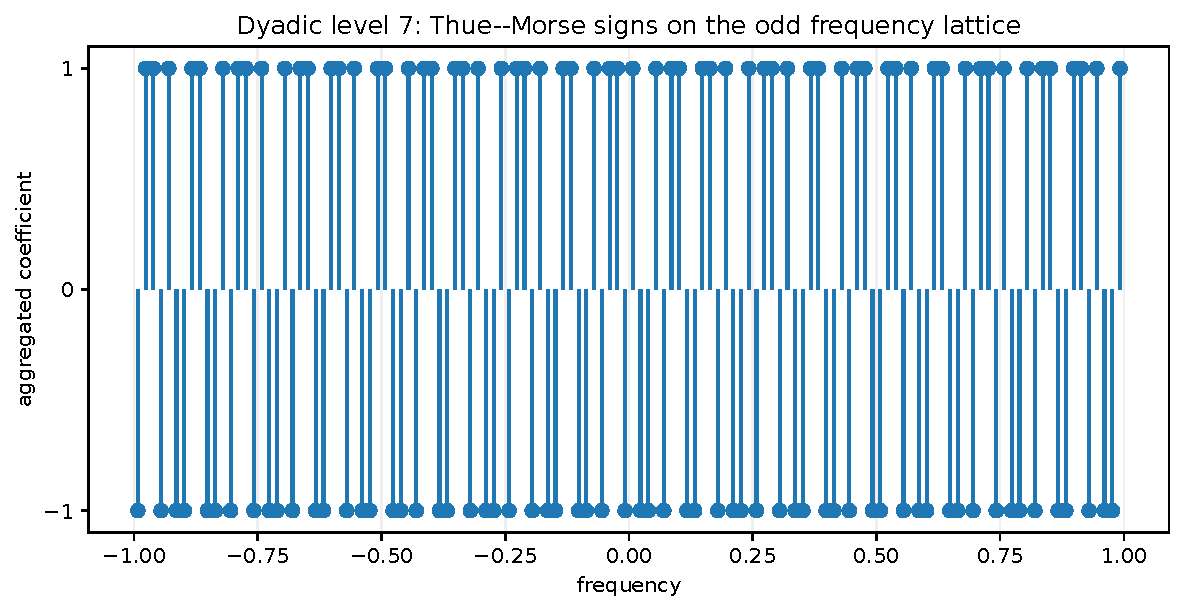
\includegraphics[width=0.92\textwidth]{data/dyadic_thue_morse_spectrum.pdf}
\caption{At level $N=7$, every odd dyadic frequency occurs once, and the
coefficient is the Thue--Morse sign $(-1)^{s_2(k)}$.}
\label{fig:dyadic-spectrum}
\end{figure}

\subsection{The minimal odd-lattice operator}

\begin{theorem}[Closed minimal dyadic ODE]
\label{thm:dyadic-minimal-ode}
Let $m=2^{N-1}$.  The gauged product $Y_N=z^N\Phi_N$ satisfies
\begin{equation}
 \boxed{
 \mathcal P_N(\D)Y_N=0,
 \qquad
 \mathcal P_N(\D):=
 \prod_{\ell=1}^{m}
 \left(\D^2+\frac{(2\ell-1)^2}{4^N}\right).}
 \label{eq:dyadic-minimal-operator}
\end{equation}
This equation has order $2^N$ and is minimal even among homogeneous linear
ODEs with rational-function coefficients.  Equivalently, $\Phi_N$ has the
minimal equation
\begin{equation}
 z^{-N}\mathcal P_N(\D)z^N\Phi_N=0.
 \label{eq:dyadic-gauged-ode}
\end{equation}
\end{theorem}
\begin{proof}
The roots of the characteristic polynomial in
\eqref{eq:dyadic-minimal-operator} are precisely
\(\ImaginaryUnit(2^N-1-2k)/2^N\), $0\le k<2^N$, the distinct exponents in
\eqref{eq:TM-exponential}.  The operator therefore annihilates $Y_N$.
Distinctness gives $r_N(1/2)=2^N$ by
\cref{cor:collision-free-classes}; minimality follows from
\cref{thm:finite-rank}.  Gauge conjugation yields
\eqref{eq:dyadic-gauged-ode} without changing the order.
\end{proof}

The first three operators are
\begin{align}
 \mathcal P_1(\D)
 &=\D^2+\frac14,\label{eq:P1}\\
 \mathcal P_2(\D)
 &=\D^4+\frac58\D^2+\frac{9}{256},\label{eq:P2}\\
 \mathcal P_3(\D)
 &=\D^8+\frac{21}{16}\D^6+\frac{987}{2048}\D^4
   +\frac{3229}{65536}\D^2+\frac{11025}{16777216}.
 \label{eq:P3}
\end{align}
The order doubles with every additional box convolution even though the finite
products converge locally uniformly to a single entire function.

\subsection{A Pochhammer factorization}

The odd squares in \eqref{eq:dyadic-minimal-operator} package into a pair of
rising factorials.

\begin{corollary}[Two-sided Pochhammer form]
\label{cor:pochhammer-operator}
With $m=2^{N-1}$ and $(a)_m=a(a+1)\cdots(a+m-1)$,
\begin{equation}
 \boxed{
 \mathcal P_N(\D)=
 2^{-(2N-2)m}
 \left(\frac12+\ImaginaryUnit2^{N-1}\D\right)_m
 \left(\frac12-\ImaginaryUnit2^{N-1}\D\right)_m.}
 \label{eq:pochhammer-operator}
\end{equation}
\end{corollary}
\begin{proof}
Pair the two factors at each $\ell$:
\begin{align*}
 &\left(\ell-\frac12+\ImaginaryUnit2^{N-1}\D\right)
  \left(\ell-\frac12-\ImaginaryUnit2^{N-1}\D\right)\\
 &\qquad=\left(\ell-\frac12\right)^2+2^{2N-2}\D^2
 =2^{2N-2}\left(\D^2+\frac{(2\ell-1)^2}{4^N}\right).
\end{align*}
Multiply over $1\le\ell\le m$.
\end{proof}

This is a literal $q$-analog bridge only in a broad structural sense: the
truncation length $m=2^{N-1}$ is geometric, while the factorization itself is
an ordinary Pochhammer product.  The genuinely $q$-dependent coefficient
calculus appears in \cref{sec:general-q-coefficients}.

\subsection{All-order Bell--Bernoulli coefficients}

Write
\begin{equation}
 \mathcal P_N(\D)=\sum_{r=0}^{m}A_{N,r}\D^{2r},
 \qquad m=2^{N-1}.
 \label{eq:operator-coeff-expansion}
\end{equation}
The coefficients are elementary symmetric polynomials in the odd squares.
Let
\begin{equation}
 S_j(m):=\sum_{\ell=1}^{m}(2\ell-1)^{2j}.
 \label{eq:odd-power-sums}
\end{equation}
We use the complete exponential Bell polynomials $\Bell_k$, normalized by
\begin{equation}
 \exp\left(\sum_{j\ge1}x_j\frac{t^j}{j!}\right)
 =\sum_{k\ge0}\Bell_k(x_1,\ldots,x_k)\frac{t^k}{k!}.
 \label{eq:Bell-normalization}
\end{equation}

\begin{theorem}[Bell--Bernoulli coefficient formula]
\label{thm:Bell-Bernoulli-operator}
For $0\le r\le m$, put $k=m-r$.  Then
\begin{equation}
 \boxed{
 A_{N,r}=4^{-Nk}\frac{1}{k!}
 \Bell_k\bigl(S_1(m),-1!S_2(m),\ldots,
              (-1)^{k-1}(k-1)!S_k(m)\bigr),}
 \label{eq:Bell-operator-coeff}
\end{equation}
where every power sum is given explicitly by the Bernoulli-polynomial value
\begin{equation}
 \boxed{
 S_j(m)=\frac{2^{2j}}{2j+1}
 \left[B_{2j+1}\!\left(m+\frac12\right)
       -B_{2j+1}\!\left(\frac12\right)\right].}
 \label{eq:Bernoulli-odd-powers}
\end{equation}
Thus every coefficient of the minimal dyadic ODE is available to arbitrary
order by a finite Bell-polynomial formula.
\end{theorem}
\begin{proof}
Expanding the product in \eqref{eq:dyadic-minimal-operator} gives
\[
 A_{N,r}=4^{-N(m-r)}e_{m-r}(1^2,3^2,\ldots,(2m-1)^2),
\]
where $e_k$ denotes the elementary symmetric polynomial.  Its generating
function is
\begin{align*}
 \sum_{k=0}^{m}e_kt^k
 &=\prod_{\ell=1}^{m}\left(1+(2\ell-1)^2t\right)\\
 &=\exp\left(\sum_{j\ge1}
       \frac{(-1)^{j-1}}{j}S_j(m)t^j\right).
\end{align*}
Comparing with \eqref{eq:Bell-normalization} proves
\eqref{eq:Bell-operator-coeff}.  Finally,
\[
 S_j(m)=2^{2j}\sum_{\ell=1}^{m}
 \left(\ell-\frac12\right)^{2j},
\]
and the standard Bernoulli-polynomial summation formula
\(
 \sum_{\ell=1}^{m}(\ell+a)^{p}
 =[B_{p+1}(m+a+1)-B_{p+1}(a+1)]/(p+1)
\)
gives \eqref{eq:Bernoulli-odd-powers} after the index is shifted.
\end{proof}

\begin{remark}[A closed coefficient pipeline]
The theorem gives an exact symbolic pipeline
\[
 \text{Bernoulli polynomials}
 \longrightarrow \text{odd power sums}
 \longrightarrow \text{Bell polynomials}
 \longrightarrow \text{minimal ODE coefficients}.
\]
It is independent of the numerical size $2^N$ of the frequency list.  This
provides a new role for the Bell--Bernoulli machinery already prominent in the
moment and endpoint parts of the repository.
\end{remark}

\subsection{Discriminant and Barnes-\texorpdfstring{$G$}{G} asymptotics}

Let $n=2^N$ and let
\begin{equation}
 \chi_N(\lambda):=
 \prod_{k=0}^{n-1}
 \left(\lambda-\frac{\ImaginaryUnit(n-1-2k)}{n}\right)
 \label{eq:dyadic-characteristic-poly}
\end{equation}
be the monic characteristic polynomial of the minimal constant-coefficient
operator.  Its roots are an arithmetic progression of step $2\ImaginaryUnit/n$.

\begin{theorem}[Exact dyadic discriminant]
\label{thm:dyadic-discriminant}
The absolute discriminant of $\chi_N$ is
\begin{equation}
 \boxed{
 \AbsoluteValue{\Disc\chi_N}
 =\left(\frac{2}{n}\right)^{n(n-1)}
   \prod_{j=1}^{n-1}(j!)^2
 =\left(\frac{2}{n}\right)^{n(n-1)}G(n+1)^2,}
 \label{eq:discriminant-Barnes}
\end{equation}
where $G$ is the Barnes $G$-function.  As $n=2^N\to\infty$,
\begin{equation}
 \log\AbsoluteValue{\Disc\chi_N}
 =n^2\left(\log2-\frac32\right)
  +n\log(\pi n)-\frac16\log n+2\zeta'(-1)
  +\BigO(n^{-2}).
 \label{eq:discriminant-asymptotic}
\end{equation}
\end{theorem}
\begin{proof}
For an arithmetic progression $a+hk$, $0\le k<n$,
\[
 \prod_{0\le j<k<n}\AbsoluteValue{h(k-j)}^2
 =\AbsoluteValue h^{n(n-1)}\prod_{k=1}^{n-1}(k!)^2.
\]
Here $\AbsoluteValue h=2/n$, which proves the first equality.  The defining integer
identity $G(n+1)=1!2!\cdots(n-1)!$ proves the second.  Substitution of the
standard expansion
\[
 \log G(n+1)=\frac{n^2}{2}\log n-\frac{3n^2}{4}
 +\frac n2\log(2\pi)-\frac1{12}\log n+\zeta'(-1)
 +\BigO(n^{-2})
\]
into \eqref{eq:discriminant-Barnes} yields
\eqref{eq:discriminant-asymptotic} after cancellation of the $n^2\log n$
terms.
\end{proof}

The negative quadratic coefficient $\log2-3/2$ shows that the discriminant
becomes exponentially small in the square of the differential rank.  Exact
rank is therefore not the whole numerical story: even the perfectly separated
dyadic lattice leads to increasingly ill-conditioned coefficient recovery in
monomial bases.

\section{General-\texorpdfstring{$q$}{q} operator coefficients from \texorpdfstring{$q$}{q}-integers and Bell polynomials}
\label{sec:general-q-coefficients}

Even when collisions occur, there is a canonical order-$2^N$ operator obtained
by retaining the entire sign-word multiset.  Define
\begin{equation}
 \mathscr P_{q,N}(\lambda):=
 \prod_{\bm\eps\in\{\pm1\}^N}
 \left(\lambda-\ImaginaryUnit\sum_{j=1}^{N}\eps_jq^j\right).
 \label{eq:universal-characteristic}
\end{equation}
It annihilates $Y_{q,N}$.  It is minimal precisely at full-rank parameters; at
an overlap parameter the minimal polynomial is obtained by retaining each
nonzero aggregated frequency once.

\begin{proposition}[Scale recursion]
\label{prop:universal-recursion}
The universal characteristic polynomials satisfy
\begin{equation}
 \boxed{
 \mathscr P_{q,N+1}(\lambda)=
 \mathscr P_{q,N}(\lambda-\ImaginaryUnit q^{N+1})
 \mathscr P_{q,N}(\lambda+\ImaginaryUnit q^{N+1}).}
 \label{eq:universal-recursion}
\end{equation}
\end{proposition}
\begin{proof}
Every level-$(N+1)$ frequency is a level-$N$ frequency plus or minus
$q^{N+1}$.  Split the product according to the last sign.
\end{proof}

The coefficients can also be built from cumulants.  Let $B_{2r}$ denote the
Bernoulli numbers with $B_2=1/6$, and write
\begin{equation}
 [N]_x:=\frac{1-x^N}{1-x}.
 \label{eq:q-integer}
\end{equation}

\begin{theorem}[$q$-integer cumulants of the frequency multiset]
\label{thm:q-cumulants}
For the Rademacher sum $W_{q,N}$ in \eqref{eq:rademacher-sum}, all odd
cumulants vanish and
\begin{equation}
 \boxed{
 \kappa_{2r}(W_{q,N})=
 \frac{2^{2r}(2^{2r}-1)B_{2r}}{2r}
 q^{2r}[N]_{q^{2r}}.}
 \label{eq:q-cumulants}
\end{equation}
Consequently, all raw moments of the frequency multiset are
\begin{equation}
 \Expectation W_{q,N}^k=
 \Bell_k\bigl(0,\kappa_2,0,\kappa_4,\ldots,\kappa_k\bigr),
 \label{eq:q-frequency-moments}
\end{equation}
and the power sums of the roots of \eqref{eq:universal-characteristic} are
\begin{equation}
 p_k:=\sum_{\bm\eps}
 \left(\ImaginaryUnit\omega(\bm\eps)\right)^k
 =2^N\ImaginaryUnit^k\Expectation W_{q,N}^k.
 \label{eq:root-power-sums}
\end{equation}
Newton's identities, equivalently a second Bell-polynomial transform, recover
every coefficient of $\mathscr P_{q,N}$ from these $p_k$.
\end{theorem}
\begin{proof}
Independence gives
\begin{equation}
 \log\Expectation\EulerE^{tW_{q,N}}=
 \sum_{j=1}^{N}\log\cosh(tq^j).
 \label{eq:logcosh-sum}
\end{equation}
The Bernoulli expansion
\begin{equation}
 \log\cosh x=
 \sum_{r\ge1}
 \frac{2^{2r}(2^{2r}-1)B_{2r}}{2r(2r)!}x^{2r}
 \label{eq:logcosh-Bernoulli}
\end{equation}
shows that the $(2r)$th cumulant is the displayed Bernoulli factor times
$\sum_{j=1}^{N}q^{2rj}=q^{2r}[N]_{q^{2r}}$.  The moment--cumulant formula is
exactly \eqref{eq:q-frequency-moments}.  Summing the $k$th powers over all
$2^N$ equally weighted sign words gives \eqref{eq:root-power-sums}; Newton's
identities are standard.
\end{proof}

\begin{corollary}[Full-rank coefficient formula]
\label{cor:full-rank-q-coeff}
If $q$ is not a root of a nonzero polynomial in $\mathscr L_{N-1}$, then
\eqref{eq:universal-characteristic} is the minimal characteristic polynomial
of $Y_{q,N}$.  Hence \cref{thm:q-cumulants} is an all-order formula for the
coefficients of the minimal ODE in terms of Bernoulli numbers, complete Bell
polynomials, and the finite $q$-integers $[N]_{q^{2r}}$.
\end{corollary}
\begin{proof}
The hypothesis gives full rank by \cref{thm:full-rank-criterion}; therefore all
$2^N$ roots in \eqref{eq:universal-characteristic} are distinct and required
by \cref{thm:finite-rank}.
\end{proof}

This combines four strands usually treated separately: geometric scaling,
Rademacher convolutions, Bernoulli-number cumulants, and reconstruction of the
differential operator by Bell polynomials.

\section{The inverse-golden-ratio overlap: the first rank defect}
\label{sec:golden}

Let
\begin{equation}
 q=\varphi^{-1}=\frac{\sqrt5-1}{2},
 \qquad q^2+q=1.
 \label{eq:golden-q}
\end{equation}
Then $q-q^2-q^3=q(1-q-q^2)=0$.  The corresponding collision appears at the
first possible nontrivial level.

\begin{proposition}[Exact level-three golden defect]
\label{prop:golden-rank6}
At $q=\varphi^{-1}$,
\begin{equation}
 r_1(q)=2,
 \qquad r_2(q)=4,
 \qquad \boxed{r_3(q)=6.}
 \label{eq:golden-ranks-first}
\end{equation}
The two sign words $(+,-,-)$ and $(-,+,+)$ both have frequency zero and have
opposite aggregate signs, so the central atom cancels completely.  The six
surviving frequencies are
\begin{equation}
 \pm2q,\qquad \pm2q^2,\qquad \pm2q^3.
 \label{eq:golden-surviving-frequencies}
\end{equation}
\end{proposition}
\begin{proof}
The displayed polynomial relation gives
$q-q^2-q^3=0$ and $-q+q^2+q^3=0$.  The products of the signs are respectively
$+1$ and $-1$, hence cancellation at zero.  Direct use of $q^2=1-q$ reduces
the remaining six sign sums to the six nonzero numbers in
\eqref{eq:golden-surviving-frequencies}; they are pairwise distinct.  Apply
\cref{thm:finite-rank}.
\end{proof}

\begin{figure}[htbp]
\centering
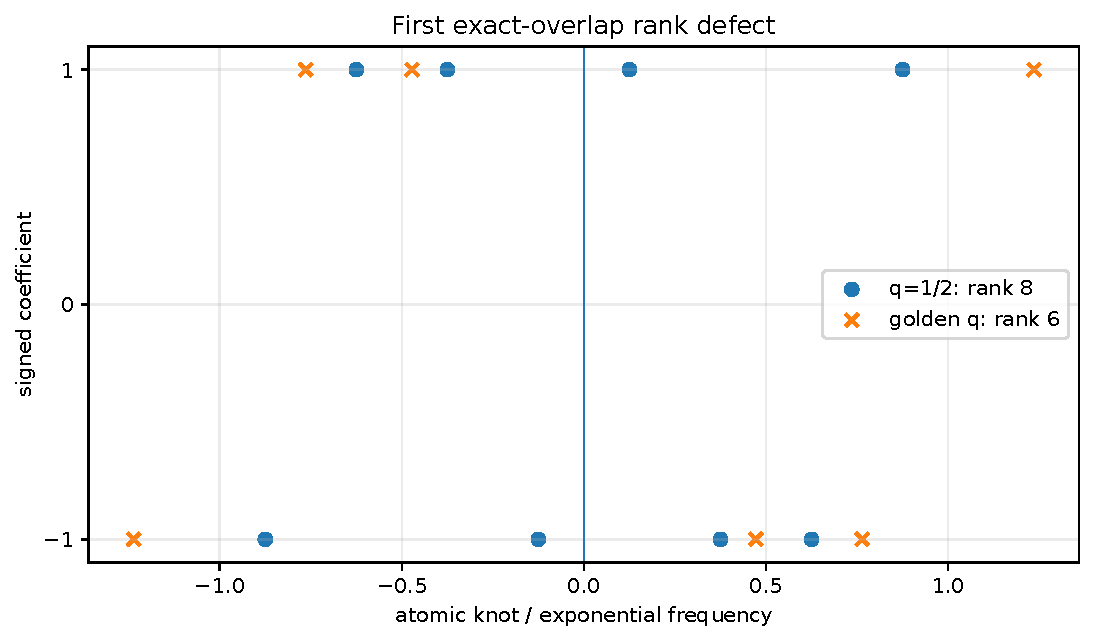
\includegraphics[width=0.86\textwidth]{data/level3_rank_defect.pdf}
\caption{The level-three dyadic product has eight signed atoms.  At the golden
parameter, the two central words collide at zero with opposite parity and
disappear, leaving differential rank six.}
\label{fig:golden-defect}
\end{figure}

By \cref{thm:rank-entropy}, even this single finite identity forces
\begin{equation}
 h_{\mathrm{hol}}(\varphi^{-1})
 \le\frac13\log6<\log2.
 \label{eq:golden-entropy-bound}
\end{equation}
Exact quadratic-field computations reveal a much more rigid pattern.

\begin{conjecture}[Golden signed-rank recurrence]
\label{conj:golden-recurrence}
Let $r_N=r_N(\varphi^{-1})$ and set $r_0=1$.  Then
\begin{equation}
 \boxed{
 r_N=2r_{N-1}-2r_{N-2}+2r_{N-3}\qquad(N\ge3),}
 \label{eq:golden-recurrence}
\end{equation}
with $r_0,r_1,r_2=1,2,4$.  Equivalently,
\begin{equation}
 \sum_{N\ge0}r_Nx^N=
 \frac{1+2x^2}{1-2x+2x^2-2x^3}.
 \label{eq:golden-rank-ogf}
\end{equation}
If true, the holonomic growth base is the real root
\begin{equation}
 \alpha=1.543689012692\ldots
 \quad\text{of}\quad
 \alpha^3-2\alpha^2+2\alpha-2=0,
 \label{eq:golden-alpha}
\end{equation}
so $h_{\mathrm{hol}}(\varphi^{-1})=\log\alpha$.
\end{conjecture}

\paragraph{Exact computational evidence.}
Arithmetic was performed in
$\IntegerNumbers[q]/(q^2+q-1)$, representing every frequency as $a+bq$ with integers
$a,b$.  Through level $25$ there was no failure of
\eqref{eq:golden-recurrence}; the ranks were
\begin{equation}
\begin{split}
1,2,4,6,8,12,20,32,48,72,112,176,272,416,640,992,{}\\
1536,2368,3648,5632,8704,13440,20736,32000,49408,76288.
\end{split}
\label{eq:golden-rank-data}
\end{equation}
Every surviving aggregate coefficient had absolute value one.  These are exact
integer statements, but they do not supply an induction invariant; hence the
recurrence remains a conjecture.

The unsigned numbers of distinct sums through the same range agree with
$F_{N+3}-1$, where $F_n$ is Fibonacci.  This suggests a finite-state normal
form for binary words under the local relation $100\leftrightarrow011$.  A
proof of the signed recurrence likely requires a refinement that records the
parity of each equivalence class, not merely its cardinality.

\begin{figure}[htbp]
\centering
\begin{subfigure}{0.49\textwidth}
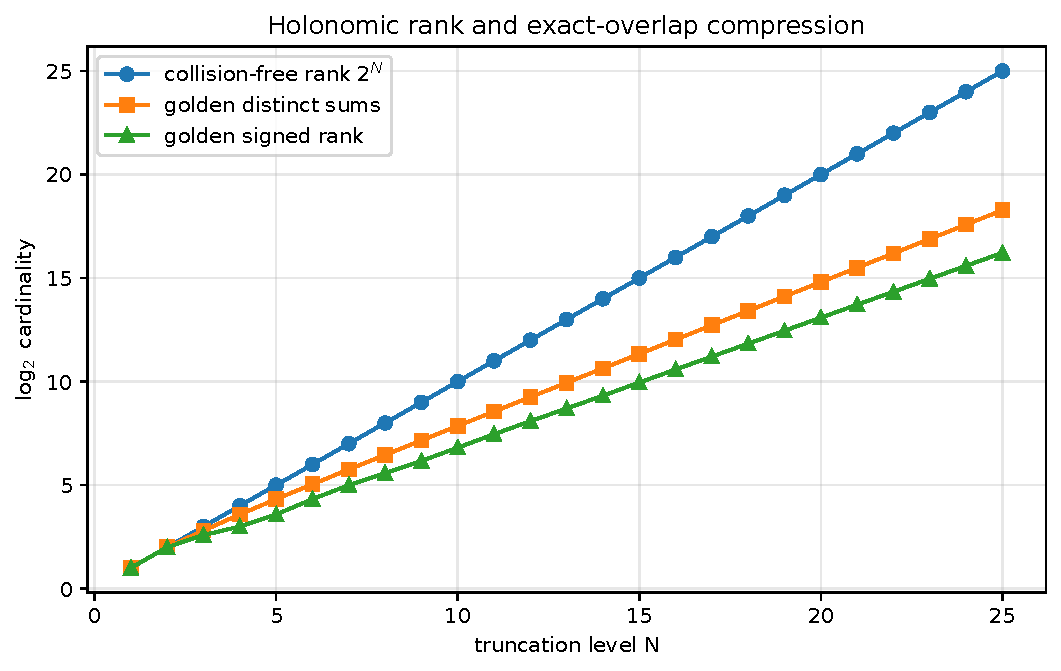
\includegraphics[width=\linewidth]{data/rank_growth.pdf}
\caption{Full, unsigned, and signed ranks.}
\end{subfigure}\hfill
\begin{subfigure}{0.49\textwidth}
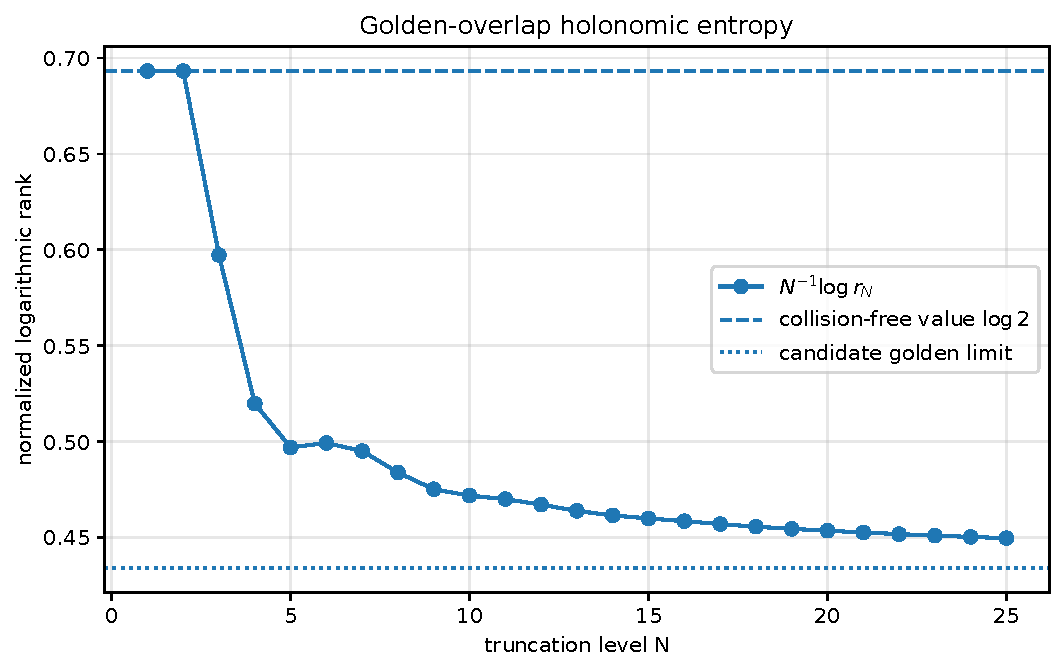
\includegraphics[width=\linewidth]{data/golden_entropy.pdf}
\caption{Convergence of normalized golden rank.}
\end{subfigure}
\caption{Exact overlap compresses both the distinct-sum set and, more strongly,
the signed holonomic support.}
\label{fig:rank-growth}
\end{figure}

\section{The infinite transform: first-order dilation, infinite differential rank}
\label{sec:infinite-nonholonomic}

\subsection{Integer-base sinc products and their divisor}

For an integer $b\ge2$, define
\begin{equation}
 \Phi_b(z):=\prod_{j=1}^{\infty}\SincRad\!\left(\frac{z}{b^j}\right).
 \label{eq:base-b-product}
\end{equation}
The product converges locally uniformly because
$\SincRad(z/b^j)=1+\BigO_K(b^{-2j})$ on every compact set $K\subset\ComplexNumbers$.  It obeys
the first-order dilation equation
\begin{equation}
 \boxed{\Phi_b(bz)=\SincRad(z)\Phi_b(z).}
 \label{eq:first-order-dilation}
\end{equation}
This is an extremely low-complexity equation in the dilation operator
$f(z)\mapsto f(bz)$.  Differential complexity behaves in the opposite way.

The zero divisor is elementary and already belongs to the repository's
spectral layer; we record it to make the new deduction self-contained.

\begin{proposition}[Integer-base zero multiplicities]
\label{prop:base-b-zeros}
The nonzero zeros of $\Phi_b$ are the points
\begin{equation}
 z=\pi bm,
 \qquad m\in\IntegerNumbers\setminus\{0\},
 \label{eq:base-b-zero-lattice}
\end{equation}
and
\begin{equation}
 \ord_{z=\pi bm}\Phi_b=1+\nu_b(m),
 \label{eq:base-b-zero-order}
\end{equation}
where $\nu_b(m)=\max\{k:b^k\mid m\}$.
\end{proposition}
\begin{proof}
The $j$th factor vanishes at $z=\pi nb^j$, $n\ne0$, and all its nonzero zeros
are simple.  At $z=\pi bm$, the factor indexed by $j$ vanishes exactly when
$b^{j-1}$ divides $m$, namely for
$1\le j\le1+\nu_b(m)$.  No other factor vanishes there.
\end{proof}

\subsection{Non-D-finiteness from unbounded multiplicity}

\begin{theorem}[The infinite sinc product is not D-finite]
\label{thm:Phi-not-Dfinite}
For every integer $b\ge2$, the entire function $\Phi_b$ is not D-finite over
$\ComplexNumbers(z)$.  In particular, it is transcendental over $\ComplexNumbers(z)$.
\end{theorem}
\begin{proof}
Suppose $\Phi_b$ satisfied an order-$r$ equation
\eqref{eq:Dfinite}, with leading polynomial $p_r\ne0$.  The zeros
$z_k=\pi b^{k+1}$ have multiplicities $k+1$ by
\cref{prop:base-b-zeros}.  For infinitely many $k\ge r$, $p_r(z_k)\ne0$
because a nonzero polynomial has only finitely many zeros.  At such an ordinary
point, $\Phi_b$ has zero multiplicity at least $r$, contradicting
\cref{lem:zero-multiplicity}.  Algebraic functions are D-finite, so
non-D-finiteness implies transcendence over $\ComplexNumbers(z)$.
\end{proof}

\begin{corollary}[A locally uniform limit leaves the D-finite category]
\label{cor:Dfinite-limit-failure}
For $b=2$, every truncation $\Phi_N$ is D-finite of exact rank $2^N$, and
$\Phi_N\to\Phi_2$ locally uniformly on $\ComplexNumbers$, but the limit is not D-finite.
Thus neither D-finiteness nor bounded differential rank is preserved under this
natural locally uniform approximation.
\end{corollary}
\begin{proof}
Finite-rank D-finiteness is \cref{thm:dyadic-minimal-ode}; local uniform
convergence follows from the product estimate above; non-D-finiteness is
\cref{thm:Phi-not-Dfinite}.
\end{proof}

\begin{remark}[Difference order versus differential order]
Equation \eqref{eq:first-order-dilation} has order one in a dilation Ore
algebra, while no finite-order linear differential operator over $\ComplexNumbers(z)$
annihilates the same function.  The Fabius--Rvachev transform is therefore a
particularly explicit separator between dilation-holonomic and
differential-holonomic behavior.
\end{remark}

\subsection{Escape from every finite dyadic trigonometric field}

For $M\ge0$, let
\begin{equation}
 \mathcal T_M:=\ComplexNumbers\!\left(z,\EulerE^{\ImaginaryUnit z/2^M}\right).
 \label{eq:trig-field}
\end{equation}
These fields form an increasing tower and are stable under $\D$.  The finite
logarithmic derivatives belong to it:
\begin{equation}
 g_N(z):=\frac{\Phi_N'(z)}{\Phi_N(z)}
 =\sum_{j=1}^{N}
 \left(2^{-j}\cot\!\left(\frac{z}{2^j}\right)-\frac1z\right)
 \in\mathcal T_N.
 \label{eq:finite-log-derivative}
\end{equation}
Let $g=\Phi_2'/\Phi_2$.  Its pole at $2\pi m$ is simple and has residue
$1+\nu_2(m)$.

We first isolate a rational-function lemma.

\begin{lemma}[Residues along a periodic rational curve]
\label{lem:rational-residues}
Fix $M\ge0$ and let
$R(z,w)\in\ComplexNumbers(z,w)$.  Suppose $R(z,\EulerE^{\ImaginaryUnit z/2^M})$ has a simple pole at
$z_n=2\pi2^Mn$ for all sufficiently large positive integers $n$.  Then its
residue at $z_n$ agrees, outside a finite exceptional set, with a rational
function of $n$.
\end{lemma}
\begin{proof}
Expand $R$ as a Laurent series at the divisor $w=1$ over the coefficient field
$\ComplexNumbers(z)$:
\begin{equation}
 R(z,w)=\sum_{k=-s}^{\infty}A_k(z)(w-1)^k,
 \qquad A_{-s}\ne0,
 \label{eq:Laurent-w1}
\end{equation}
where the principal part is finite and every $A_k(z)$ is rational.  A rational
factor depending only on $z$ can create poles at only finitely many $z_n$;
therefore $s\ge1$.  Since
\begin{equation}
 \EulerE^{\ImaginaryUnit z/2^M}-1
 =\frac{\ImaginaryUnit}{2^M}(z-z_n)+\BigO((z-z_n)^2)
 \label{eq:exp-local}
\end{equation}
near $z_n$, the generic pole order after substitution is $s$.  The coefficient
$A_{-s}(z_n)$ can vanish for only finitely many $n$ unless it is identically
zero.  The assumed simple poles therefore force $s=1$.  Their residues are
\begin{equation}
 \frac{2^M}{\ImaginaryUnit}A_{-1}(2\pi2^Mn),
 \label{eq:rational-residue-n}
\end{equation}
which is a rational function of $n$.
\end{proof}

\begin{theorem}[Trigonometric-field escape]
\label{thm:field-escape}
For every $M\ge0$,
\begin{equation}
 \boxed{
 \frac{\Phi_2'}{\Phi_2}\notin\mathcal T_M.}
 \label{eq:log-derivative-escape}
\end{equation}
Consequently,
\begin{equation}
 \Phi_2\notin\bigcup_{M\ge0}\mathcal T_M.
 \label{eq:Phi-field-escape}
\end{equation}
Thus the infinite logarithmic derivative is not a rational expression in $z$
and trigonometric functions from any fixed finite dyadic frequency level,
even though every finite truncation has such an expression.
\end{theorem}
\begin{proof}
Suppose $g=\Phi_2'/\Phi_2$ belonged to $\mathcal T_M$.  At
$z_n=2\pi2^Mn$ its residue is
\begin{equation}
 1+\nu_2(2^Mn)=M+1+\nu_2(n).
 \label{eq:residue-ruler}
\end{equation}
By \cref{lem:rational-residues}, this would agree eventually with a rational
function $S(n)\in\ComplexNumbers(n)$.  On all sufficiently large odd integers $n$, the
right-hand side of \eqref{eq:residue-ruler} equals $M+1$.  Hence the rational
function $S(n)-(M+1)$ has infinitely many zeros and is identically zero.  But
at $n=2^k$ the required residue is $M+1+k$, a contradiction.

If $\Phi_2\in\mathcal T_M$, then stability under differentiation and division
would imply $\Phi_2'/\Phi_2\in\mathcal T_M$, already excluded.
\end{proof}

\begin{remark}
The proof uses not merely the existence of infinitely many zeros but the
non-rational arithmetic variation of their multiplicities along the lattice.
The ruler function $1+\nu_2(n)$ is therefore an obstruction to finite-level
trigonometric closed form.
\end{remark}

\section{Moment, cumulant, and reciprocal sequences are not P-recursive}
\label{sec:moment-nonprecursive}

\subsection{The moment-generating function}

For the dyadic random variable $X$ in \eqref{eq:rvachev-random-series}, define
\begin{equation}
 M(t):=\Expectation\EulerE^{tX}
 =\prod_{j=1}^{\infty}
 \frac{\sinh(t/2^j)}{t/2^j}
 =\Phi_2(-\ImaginaryUnit t).
 \label{eq:MGF}
\end{equation}
Let
\begin{equation}
 M(t)=\sum_{n\ge0}\mu_n\frac{t^n}{n!},
 \qquad
 K(t):=\log M(t)=\sum_{n\ge1}\kappa_n\frac{t^n}{n!},
 \qquad
 \frac1{M(t)}=\sum_{n\ge0}\rho_n\frac{t^n}{n!}.
 \label{eq:three-EGFs}
\end{equation}
Here $\mu_n$ are moments, $\kappa_n$ are cumulants, and $\rho_n$ are the
signed reciprocal-moment coefficients.  Symmetry makes all odd terms vanish.

The cumulants have a familiar exact Bernoulli formula, included both for
reference and to expose the Bell-polynomial consequences.

\begin{proposition}[Rvachev cumulants]
\label{prop:Rvachev-cumulants}
For $r\ge1$,
\begin{equation}
 \boxed{
 \kappa_{2r}=
 \frac{2^{2r}B_{2r}}{2r(2^{2r}-1)},
 \qquad \kappa_{2r+1}=0.}
 \label{eq:Rvachev-cumulants}
\end{equation}
Furthermore,
\begin{equation}
 \mu_n=\Bell_n(\kappa_1,\ldots,\kappa_n),
 \qquad
 \rho_n=\Bell_n(-\kappa_1,\ldots,-\kappa_n).
 \label{eq:moment-Bell}
\end{equation}
\end{proposition}
\begin{proof}
The standard expansion
\begin{equation}
 \log\frac{\sinh x}{x}
 =\sum_{r\ge1}
 \frac{2^{2r}B_{2r}}{2r(2r)!}x^{2r}
 \label{eq:logsinh-expansion}
\end{equation}
gives
\begin{align*}
 K(t)
 &=\sum_{j\ge1}\log\frac{\sinh(t/2^j)}{t/2^j}\\
 &=\sum_{r\ge1}
 \frac{2^{2r}B_{2r}}{2r(2r)!}
 \left(\sum_{j\ge1}2^{-2rj}\right)t^{2r}\\
 &=\sum_{r\ge1}
 \frac{2^{2r}B_{2r}}{2r(2r)!(2^{2r}-1)}t^{2r}.
\end{align*}
Comparison with \eqref{eq:three-EGFs} proves
\eqref{eq:Rvachev-cumulants}.  Since $M=\exp K$ and $M^{-1}=\exp(-K)$,
the two Bell formulae follow from \eqref{eq:Bell-normalization}.
\end{proof}

\subsection{Three non-P-recursive rational sequences}

\begin{theorem}[Moment and Bell-sequence obstruction]
\label{thm:moment-not-P-recursive}
None of the three sequences
\begin{equation}
 (\mu_n)_{n\ge0},\qquad
 (\kappa_n)_{n\ge0},\qquad
 (\rho_n)_{n\ge0}
 \label{eq:three-sequences}
\end{equation}
is P-recursive.  Their even subsequences
$(\mu_{2n})$, $(\kappa_{2n})$, and $(\rho_{2n})$ are likewise not
P-recursive.
\end{theorem}
\begin{proof}
The MGF $M(t)=\Phi_2(-\ImaginaryUnit t)$ is not D-finite by
\cref{thm:Phi-not-Dfinite}.  If $(\mu_n)$ were P-recursive, then
$(\mu_n/n!)$ would also be P-recursive: substitute
$\mu_{n+j}=(n+j)![t^{n+j}]M$ into a recurrence and clear shifted factorials.
Stanley's equivalence would make $M$ D-finite, a contradiction.

The function $M$ has infinitely many zeros, inherited from $\Phi_2$.
Therefore $1/M$ has infinitely many poles and is not D-finite by
\cref{lem:finite-singular-locus}.  This excludes P-recursiveness of
$(\rho_n)$ by the same factorial argument.

If $K$ were D-finite, then $K'=M'/M$ would be D-finite.  But $M'/M$ has a
simple pole at every zero of $M$, with residue equal to its multiplicity, hence
infinitely many finite-plane poles.  This contradicts
\cref{lem:finite-singular-locus}.  Thus $(\kappa_n)$ is not P-recursive.

Finally suppose, for example, that $(\mu_{2n})$ were P-recursive.  Then
$c_n=\mu_{2n}/(2n)!$ would be P-recursive after clearing the hypergeometric
factor $(2n)!$ in any recurrence.  The ordinary series
$C(z)=\sum c_nz^n$ would be D-finite, and D-finiteness is preserved under the
algebraic substitution $z=t^2$.  But $C(t^2)=M(t)$, a contradiction.  The same
argument applies to the other two even subsequences.
\end{proof}

\begin{corollary}[A non-P-recursive Bernoulli-number specialization]
\label{cor:Bernoulli-specialization-nonP}
The explicit rational sequence
\begin{equation}
 \left(
 \frac{2^{2n}B_{2n}}{2n(2^{2n}-1)}
 \right)_{n\ge1}
 \label{eq:weighted-Bernoulli-sequence}
\end{equation}
is not P-recursive.
\end{corollary}
\begin{proof}
It is the even cumulant sequence in \eqref{eq:Rvachev-cumulants}; apply
\cref{thm:moment-not-P-recursive}.
\end{proof}

\begin{remark}[Why explicit does not mean holonomic]
The cumulants have a one-line Bernoulli formula, and the moments and reciprocal
coefficients have finite Bell-polynomial formulae at each order.  Nevertheless,
no fixed polynomial-coefficient recurrence controls any of the resulting
infinite sequences.  The obstruction is global analytic structure: infinitely
many singularities for $K'$ and $1/M$, and unbounded zero multiplicity for
$M$.
\end{remark}

\subsection{The functions \texorpdfstring{$F$ and $\RvachevUp$}{F and up} themselves}

Fabius's original example is nowhere analytic on its active interval
\cite{Fabius}; the repository develops stronger variants and iterated
consequences.  This immediately has a holonomic interpretation.

\begin{corollary}[The Fabius and up functions are not D-finite]
\label{cor:F-up-not-Dfinite}
No nonzero polynomial-coefficient linear ODE can hold for $F$ on an interval
containing a nontrivial subinterval of $(0,1)$.  The same is true for $\RvachevUp$ on
an interval meeting $(-1,1)$ nontrivially.
\end{corollary}
\begin{proof}
A solution of a polynomial-coefficient linear ODE is real analytic at every
ordinary point; only the finitely many roots of the leading coefficient can be
singular.  The function $F$ is nowhere analytic on $(0,1)$, so such an ODE is
impossible.  Relation \eqref{eq:F-up} transfers the same obstruction to either
active half of $\RvachevUp$.
\end{proof}

\section{Deep dyadic Fabius samples and P-recursiveness}
\label{sec:deep-samples}

The previous section used the Fourier transform.  A different obstruction comes
directly from the endpoint self-differential equation and applies to the exact
sample sequence most prominent in the arithmetic theory.

For fixed $c>0$, define, after any harmless finite initial prefix,
\begin{equation}
 a_n(c):=F(c2^{-n}).
 \label{eq:deep-sample}
\end{equation}
For all sufficiently large $n$, the argument lies in $(0,1/2]$.  Integrating
\eqref{eq:fabius-diff} from $0$ to $x$ and using $F(0)=0$ gives the exact
Volterra identity
\begin{equation}
 F(x)=\int_0^{2x}F(u)\Differential u,
 \qquad 0\le x\le\frac12.
 \label{eq:F-Volterra}
\end{equation}
Monotonicity now forces a rapidly contracting ratio.

\begin{lemma}[Supergeometric one-step bound]
\label{lem:sample-ratio}
For every fixed $c>0$ and all sufficiently large $n$,
\begin{equation}
 0<a_{n+1}(c)\le c2^{-n}a_n(c).
 \label{eq:sample-ratio}
\end{equation}
More generally, for every fixed $j\ge1$,
\begin{equation}
 \frac{a_{n+j}(c)}{a_n(c)}
 \le c^j2^{-jn-j(j-1)/2}.
 \label{eq:sample-ratio-iterated}
\end{equation}
\end{lemma}
\begin{proof}
Apply \eqref{eq:F-Volterra} with $x=c2^{-n-1}$:
\[
 a_{n+1}(c)=\int_0^{c2^{-n}}F(u)\Differential u.
\]
Since $F$ is increasing and positive on $(0,1)$, the integral is positive and
at most $c2^{-n}F(c2^{-n})$.  Iterating this estimate proves
\eqref{eq:sample-ratio-iterated}.
\end{proof}

\begin{theorem}[No P-recursion for deep dyadic samples]
\label{thm:deep-samples-not-P}
For every $c>0$, the sequence $(F(c2^{-n}))_{n\ge0}$ is not P-recursive.  In
particular, the exact rational sequence
\begin{equation}
 \boxed{\bigl(F(2^{-n})\bigr)_{n\ge0}}
 \label{eq:exact-dyadic-sequence}
\end{equation}
is not P-recursive.
\end{theorem}
\begin{proof}
A finite change of initial terms does not affect P-recursiveness, so assume all
arguments are in $(0,1/2]$.  Suppose
\begin{equation}
 \sum_{j=0}^{r}p_j(n)a_{n+j}(c)=0
 \label{eq:assumed-sample-recurrence}
\end{equation}
for all sufficiently large $n$, with polynomial coefficients not all zero.
Let $j_0$ be the least index for which $p_{j_0}$ is nonzero.  Divide by the
positive number $a_{n+j_0}(c)$.  By
\eqref{eq:sample-ratio-iterated}, for $j>j_0$,
\begin{equation}
 \frac{a_{n+j}(c)}{a_{n+j_0}(c)}
 =\BigO\!\left(2^{-(j-j_0)n}\right).
 \label{eq:later-samples-small}
\end{equation}
Therefore \eqref{eq:assumed-sample-recurrence} implies
\begin{equation}
 p_{j_0}(n)=
 -\sum_{j=j_0+1}^{r}p_j(n)
   \frac{a_{n+j}(c)}{a_{n+j_0}(c)}
 \longrightarrow0.
 \label{eq:polynomial-to-zero}
\end{equation}
The right-hand side tends to zero because a polynomial times an exponentially
decaying sequence tends to zero.  A nonzero polynomial cannot tend to zero
along the positive integers.  This contradiction proves the theorem.

Arias de Reyna proved that $F$ takes rational values at dyadic arguments and
established strong denominator and integrality properties
\cite{AriasDefinition,AriasArithmetic}.  Hence the specialization $c=1$ is an
exact rational, not merely numerical, example.
\end{proof}

\subsection{All fixed derivative orders}

Repeated differentiation of \eqref{eq:fabius-diff} gives a triangular scaling
law near the endpoint.

\begin{lemma}[Endpoint derivative scaling]
\label{lem:derivative-scaling}
For every integer $m\ge0$ and $0\le x\le2^{-m}$,
\begin{equation}
 F^{(m)}(x)=2^{m(m+1)/2}F(2^mx).
 \label{eq:derivative-scaling}
\end{equation}
\end{lemma}
\begin{proof}
The assertion is trivial for $m=0$ and is \eqref{eq:fabius-diff} for $m=1$.
If it holds for $m$, differentiate on $0\le x\le2^{-(m+1)}$:
\begin{align*}
 F^{(m+1)}(x)
 &=2^{m(m+1)/2}2^mF'(2^mx)\\
 &=2^{m(m+1)/2+m+1}F(2^{m+1}x)\\
 &=2^{(m+1)(m+2)/2}F(2^{m+1}x).
\end{align*}
\end{proof}

\begin{corollary}[Derivative sample obstruction]
\label{cor:derivative-samples-not-P}
For every fixed $m\ge0$ and $c>0$, the sequence
\begin{equation}
 \bigl(F^{(m)}(c2^{-n})\bigr)_{n\ge0}
 \label{eq:derivative-sample-sequence}
\end{equation}
is not P-recursive.
\end{corollary}
\begin{proof}
For sufficiently large $n$, \eqref{eq:derivative-scaling} gives
\[
 F^{(m)}(c2^{-n})=2^{m(m+1)/2}F(c2^{-(n-m)}).
\]
This is a nonzero constant multiple and finite shift of the sequence in
\cref{thm:deep-samples-not-P}.
\end{proof}

\subsection{An entire generating function of order zero}

Define the ordinary generating function
\begin{equation}
 A_c(z):=\sum_{n=0}^{\infty}F(c2^{-n})z^n,
 \label{eq:sample-OGF}
\end{equation}
where any clamped or omitted finite prefix is immaterial.

\begin{theorem}[Order-zero sample generating function]
\label{thm:sample-OGF-order-zero}
For every $c>0$, $A_c$ is a nonpolynomial entire function of order zero.  More
precisely, with
$M_c(r)=\max_{\AbsoluteValue z=r}\AbsoluteValue{A_c(z)}$,
\begin{equation}
 \log M_c(r)
 \le\frac{(\log r)^2}{2\log2}+\BigO(\log r)
 \qquad(r\to\infty).
 \label{eq:sample-OGF-growth}
\end{equation}
It is not D-finite.
\end{theorem}
\begin{proof}
Iteration of \eqref{eq:sample-ratio} yields constants $C_0,C_1>0$ such that
\begin{equation}
 0<a_n(c)\le C_0C_1^n2^{-n(n-1)/2}.
 \label{eq:sample-coefficient-upper}
\end{equation}
The ratio test gives infinite radius of convergence.  For $r\ge1$,
\begin{align*}
 M_c(r)
 &\le C_0\sum_{n\ge0}
 \exp\left[-\frac{\log2}{2}n^2
 +n\left(\log(C_1r)+\frac{\log2}{2}\right)\right].
\end{align*}
Completing the square bounds this Gaussian sum by a polynomial factor times
\[
 \exp\left(
 \frac{(\log(C_1r)+\frac12\log2)^2}{2\log2}
 \right),
\]
which proves \eqref{eq:sample-OGF-growth}.  Consequently
\[
 \limsup_{r\to\infty}
 \frac{\log\log M_c(r)}{\log r}=0,
\]
so the order is zero.  Every coefficient is eventually positive, hence the
function is not a polynomial.  Finally, if $A_c$ were D-finite, its coefficient
sequence would be P-recursive, contrary to
\cref{thm:deep-samples-not-P}.
\end{proof}

\begin{remark}[Endpoint asymptotics enter at the next order]
The leading log-square bound in \eqref{eq:sample-OGF-growth} is only an upper
estimate.  The repository's corrected endpoint transseries for $F(x)$ as
$x\downarrow0$, with Lambert--$W$ carrier and a nonconstant dyadic periodic
factor, should permit a saddle-point expansion of $A_c(r)$ with logarithmic
periodicity.  This is formulated as a future problem in
\cref{problem:sample-OGF-asymptotic}.
\end{remark}

\section{Numerical experiments and reproducibility}
\label{sec:numerics}

All experiments are contained in the commented script
\texttt{frontier\_experiments.py}.  The rank computations use exact arithmetic:
$\RationalNumbers$ for rational $q$, and integer pairs $a+bq$ modulo $q^2+q-1$ for the golden
parameter.  Floating point is used only to order already deduplicated algebraic
numbers for plotting, and to display high-precision residuals.

\subsection{Rank table}

\begin{table}[htbp]
\centering
\caption{Exact ranks and unsigned distinct-sum counts at selected levels.}
\label{tab:ranks}
\begin{tabular}{rrrrr}
\toprule
$N$ & $r_N(1/2)$ & $r_N(2/3)$ & $r_N(\varphi^{-1})$
    & $d_N(\varphi^{-1})$\\
\midrule
1  & 2      & 2      & 2    & 2\\
2  & 4      & 4      & 4    & 4\\
3  & 8      & 8      & 6    & 7\\
4  & 16     & 16     & 8    & 12\\
5  & 32     & 32     & 12   & 20\\
6  & 64     & 64     & 20   & 33\\
8  & 256    & 256    & 48   & 88\\
10 & 1024   & 1024   & 112  & 232\\
12 & 4096   & 4096   & 272  & 609\\
16 & 65536  & 65536  & 1536 & 4180\\
20 & 1048576& 1048576& 8704 & 28656\\
25 & 33554432&33554432&76288 & 317810\\
\bottomrule
\end{tabular}
\end{table}

The rational parameter $2/3$ stays at full exact rank, as proved by the
rational-root argument in \cref{cor:collision-free-classes}.  Nevertheless its
frequency separation shrinks faster than in the dyadic case, illustrating that
exact rank and numerical conditioning are distinct invariants.

\begin{figure}[htbp]
\centering
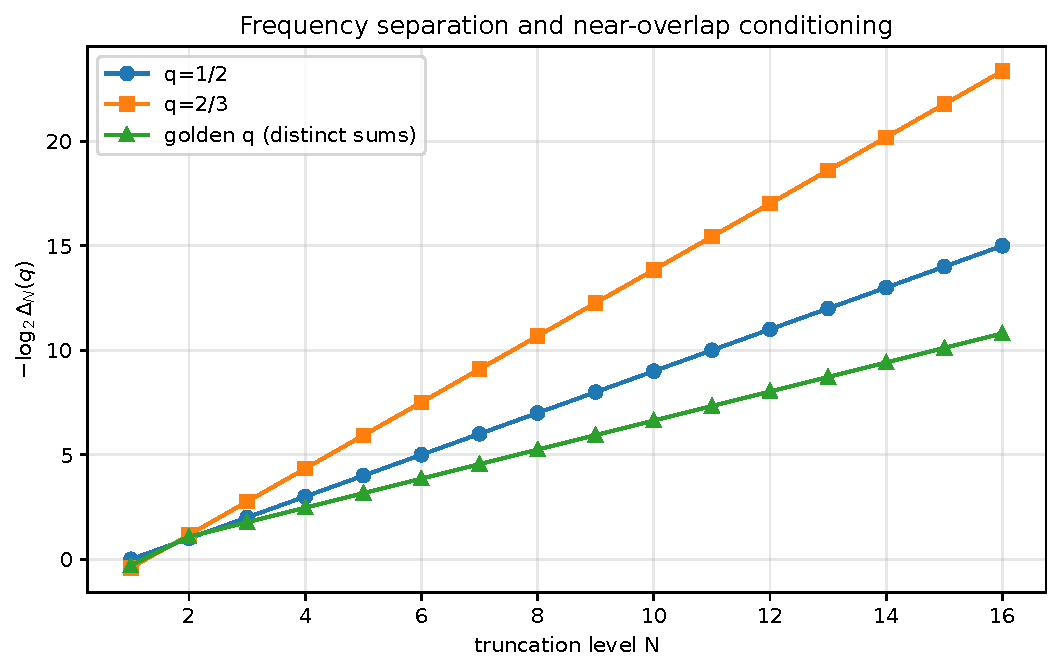
\includegraphics[width=0.88\textwidth]{data/frequency_separation.pdf}
\caption{Minimum spacing of distinct signed sums.  For $q=1/2$, the exact law is
$\Delta_N=2^{1-N}$.  The $q=2/3$ and golden curves were computed in exact
rational or quadratic-field arithmetic before numerical display.}
\label{fig:frequency-separation}
\end{figure}

\subsection{Operator residual and discriminant checks}

The script constructs $\mathcal P_N$ with exact SymPy rationals and evaluates
$\mathcal P_N(\D)Y_N$ by differentiating the Thue--Morse exponential sum term
by term at $120$ decimal digits.  For $1\le N\le5$ and the test points
$z=0.37,1.1,2.7$, the largest relative residual was below
\begin{equation}
 8.4\times10^{-122}.
 \label{eq:residual-bound}
\end{equation}
This is a consistency check, not part of the proof of minimality.

The Barnes-$G$ discriminant formula was evaluated through $N=12$ using
\eqref{eq:discriminant-Barnes}; the difference from the asymptotic
\eqref{eq:discriminant-asymptotic} decays at the expected inverse-square rate.
Complete tables are included under \texttt{data/}.

\subsection{Reproduction command}

From the unpacked archive, run
\begin{lstlisting}[language=bash]
python frontier_experiments.py --output-dir data
latexmk -pdf -interaction=nonstopmode fabius_holonomic_frontiers.tex
\end{lstlisting}
The script records the tested package versions in
\texttt{NUMERICAL\_README.md}; \texttt{requirements.txt} gives the minimal
Python dependencies.

\section{Conjectures and promising research directions}
\label{sec:future}

\subsection{Proving the golden finite-state recurrence}

\begin{problem}[A parity-sensitive normalization automaton]
\label{problem:golden-automaton}
Construct a finite-state transducer for sign words modulo
$q^2+q-1=0$ that tracks both the represented frequency and the parity weight
$\prod\eps_j$.  Use it to prove or refute
\cref{conj:golden-recurrence}, and determine whether every surviving aggregate
coefficient is always $\pm1$.
\end{problem}

The unsigned relation $100\leftrightarrow011$ suggests a canonical-word
language, but signed cancellation requires more information than a normal form
for values.  A successful automaton should yield a rational generating
function for $r_N$, a finite matrix whose Perron root is the rank growth base,
and perhaps a complete classification of local knot cancellations in the
finite splines.

\subsection{Differential transcendence}

\begin{conjecture}[Differential transcendence of the Rvachev transform]
\label{conj:differential-transcendence}
For every integer $b\ge2$, the function
\begin{equation}
 \Phi_b(z)=\prod_{j\ge1}\SincRad(z/b^j)
 \label{eq:DT-conjecture-function}
\end{equation}
is differentially transcendental over $\ComplexNumbers(z)$; that is, it satisfies no
nonzero algebraic differential equation with coefficients in $\ComplexNumbers(z)$.
The same should hold for its moment-generating specialization
$\Phi_b(-\ImaginaryUnit t)$.
\end{conjecture}

\cref{thm:Phi-not-Dfinite} excludes only \emph{linear} differential equations.
The first-order dilation equation \eqref{eq:first-order-dilation} makes the
conjecture a natural target for parameterized difference Galois theory.
Existing criteria cover broad classes of shift, $q$-dilation, and Mahler
equations \cite{ArrecheDreyfusRoques,AdamczewskiDreyfusHardouinWibmer}, but the
coefficient $\SincRad z$ naturally lives in a trigonometric extension rather than
$\ComplexNumbers(z)$.  The residue obstruction in \cref{thm:field-escape} is evidence that no
finite trigonometric extension trivializes the equation.

A concrete intermediate target is to classify all differential-algebraic
solutions of
\begin{equation}
 y(2z)=\SincRad(z)y(z)
 \label{eq:dilation-DT-target}
\end{equation}
over the differential-difference field generated by
$z$ and all $\EulerE^{\ImaginaryUnit z/2^M}$.  The divisor orbit under $z\mapsto2z$ should enter
the parameterized Galois group explicitly.

\subsection{Rank entropy versus Bernoulli-convolution entropy}

\begin{conjecture}[Signed and unsigned overlap exponents]
\label{conj:rank-vs-Garsia}
Let
\begin{equation}
 h_{\mathrm{supp}}(q)=\lim_{N\to\infty}\frac1N\log d_N(q),
 \qquad
 h_{\mathrm{hol}}(q)=\lim_{N\to\infty}\frac1N\log r_N(q).
 \label{eq:two-entropies}
\end{equation}
For algebraic exact-overlap parameters, both exponents should be computable by
a finite algebraic automaton.  The signed exponent should equal the logarithm
of the spectral radius of a parity-refined overlap matrix, and should admit
inequalities in terms of the Garsia entropy of the corresponding Bernoulli
convolution.
\end{conjecture}

The theorem $h_{\mathrm{hol}}(q)<\log2$ if and only if an exact overlap occurs
is stronger than a generic upper bound but weaker than a quantitative entropy
formula.  Hochman's inverse theorem identifies superexponentially close
cylinders as the mechanism behind dimension drop and proves exact-overlap
consequences for algebraic parameters \cite{Hochman}.  The new rank entropy is
a signed algebraic statistic that may provide a tractable finite-state shadow
of that theory.

\subsection{Near-overlap conditioning and restricted-coefficient polynomials}

The exact identity \eqref{eq:separation-Littlewood} turns the smallest frequency
gap into a restricted-coefficient polynomial problem.  This suggests three
quantitative projects.
\begin{enumerate}
 \item Bound the condition number of the derivative-to-frequency Vandermonde
       matrix in terms of $\Delta_N(q)$ and the maximum frequency.
 \item For a fixed algebraic $q$ with no exact overlap, combine root-separation
       bounds with the restricted-coefficient literature
       \cite{BorweinPinner,BorweinErdelyiKos} to obtain explicit lower bounds
       for $\Delta_N(q)$.
 \item Study a numerical ``effective rank'' obtained by merging frequencies
       below a precision threshold.  Its phase changes should track near roots
       of $\{-1,0,1\}$ polynomials even when the exact rank remains $2^N$.
\end{enumerate}

\subsection{A mixed dilation--differential Ore algebra}

The finite operators $\mathcal P_N(\D)$ grow exponentially in order, while the
infinite transform has the first-order dilation equation
\eqref{eq:first-order-dilation}.  A computationally useful symbolic theory
should therefore not insist on pure differential holonomicity.

\begin{problem}[Minimal mixed operator]
\label{problem:mixed-Ore}
In the Ore algebra generated by multiplication by meromorphic functions,
$\D$, and the dilation $\sigma_bf(z)=f(bz)$, determine a canonical minimal
annihilating ideal for $\Phi_b$.  Develop closure and creative-telescoping rules
that retain the first-order dilation relation instead of expanding to the
exponentially large finite differential operators.
\end{problem}

The finite rank formulae provide test cases: truncation at level $N$ should
produce an elimination operator of exact differential order $r_N(q)$, and
exact overlaps should appear as order drops in noncommutative elimination.

\subsection{Inverse Fabius samples}

\begin{conjecture}[Non-P-recursiveness of inverse endpoint samples]
\label{conj:inverse-samples}
For every fixed $c>0$, the sequence
\begin{equation}
 b_n(c):=F^{-1}(c2^{-n})
 \label{eq:inverse-sample}
\end{equation}
for sufficiently large $n$ is not P-recursive.
\end{conjecture}

Unlike $F(c2^{-n})$, the inverse sequence decays only stretched-exponentially
in $\sqrt n$ at leading order, a scale compatible with some P-recursive
asymptotic templates.  A proof will therefore need the complete endpoint
structure, probably the nonconstant log-periodic factor in the corrected
Lambert--$W$ expansion, rather than a simple ratio argument.  One possible
route is to show that the asymptotic transseries violates the finite collection
of exponential scales allowed by Birkhoff--Trjitzinsky theory for polynomial
recurrences.

\subsection{Saddle analysis of the order-zero sample OGF}

\begin{problem}[Sharp growth of $A_c$]
\label{problem:sample-OGF-asymptotic}
Insert the all-orders endpoint expansion of $F(c2^{-n})$ into
\begin{equation}
 A_c(r)=\sum_{n\ge0}F(c2^{-n})r^n
 \label{eq:Ac-saddle-sum}
\end{equation}
and derive a complete saddle expansion as $r\to+\infty$.  Determine whether
\begin{equation}
 \log A_c(r)=\frac{(\log r)^2}{2\log2}
 +\text{lower log--log terms}
 +\mathcal Q_c(\log_2\log r)+o(1)
 \label{eq:Ac-conjectural-growth}
\end{equation}
with a nonconstant periodic function $\mathcal Q_c$.
\end{problem}

This would create a new duality between the endpoint asymptotics of $F$ and the
growth theory of an entire function of order zero.  The saddle index is of
size $\log_2 r$, while the endpoint carrier itself contains a Lambert--$W$
scale; their interaction should produce a two-level asymptotic inversion.

\subsection{Formalization targets}

Several proofs are unusually suitable for Lean formalization.
\begin{enumerate}
 \item Polynomial-exponential independence and the exact rank theorem can be
       reduced to finite-dimensional linear algebra plus polynomial
       injectivity of $\D+c$.
 \item The collision criterion is a finite equivalence on sign vectors and
       $\{-1,0,1\}$ coefficient lists.
 \item Rank submultiplicativity and Fekete's lemma give the entropy theorem.
 \item The non-D-finiteness proof needs only the ordinary-point uniqueness
       theorem and the already formalized zero multiplicities.
 \item The deep-sample obstruction is an elementary asymptotic contradiction
       from monotonicity and \eqref{eq:F-Volterra}.
\end{enumerate}
A formal development would be small relative to the existing Fabius corpus and
would certify several genuinely global negative statements that are otherwise
easy to overlook.

\section{Conclusion}
\label{sec:conclusion}

The finite and infinite sinc products sit on opposite sides of a sharp
holonomic boundary.  A finite product is an exponential polynomial after one
rational gauge, but its exact differential rank is not merely the number of
factors: it is the signed support size of a Bernoulli convolution, equivalently
the number of surviving top-order spline knots.  This turns exact overlaps
into minimal-ODE rank defects and produces a submultiplicative entropy that
detects every restricted-coefficient algebraic relation.

At the dyadic parameter, the absence of overlaps exposes the full
$2^N$-dimensional structure.  The odd frequency lattice yields a complete
minimal operator, Thue--Morse coefficients, a Pochhammer factorization,
Bell--Bernoulli coefficient formulae, and an exact Barnes-$G$ discriminant.
The infinite limit retains a first-order dilation equation but loses all finite
linear differential description.  Its zero multiplicities, arithmetic
residues, and singularity pattern force non-D-finiteness, trigonometric-field
escape, and non-P-recursiveness of several natural moment and endpoint
sequences.

The strongest open bridge is now clear: combine exact-overlap automata,
parameterized difference Galois theory, and the repository's Lambert--$W$
endpoint transseries.  That program could upgrade the present linear
non-holonomicity to differential transcendence, solve the golden rank
recurrence, and connect rank entropy to the much deeper entropy theory of
Bernoulli convolutions.

\appendix

\section{A compact theorem dependency map}
\label{app:dependency}

\begin{center}
\begin{tabularx}{\textwidth}{>{\raggedright\arraybackslash}p{0.28\textwidth}X}
\toprule
Result & Inputs\\
\midrule
Exact finite rank, \cref{thm:finite-rank}
 & Exponential expansion \eqref{eq:frequency-expansion};
   polynomial-exponential independence, \cref{lem:exp-independence}.\\
Rank--knot duality, \cref{thm:rank-knot}
 & Distributional derivative of a box; exact finite rank.\\
Full-rank criterion, \cref{thm:full-rank-criterion}
 & Difference of two sign words is $2qP(q)$ with
   $P\in\{-1,0,1\}[x]$.\\
Rank entropy, \cref{thm:rank-entropy}
 & Block factorization \eqref{eq:block-factorization}; Fekete's lemma.\\
Dyadic minimal ODE, \cref{thm:dyadic-minimal-ode}
 & Odd-lattice/Thue--Morse parametrization; exact finite rank.\\
Bell--Bernoulli coefficients, \cref{thm:Bell-Bernoulli-operator}
 & Newton/Bell transform and Bernoulli polynomial power sums.\\
Infinite non-D-finiteness, \cref{thm:Phi-not-Dfinite}
 & Existing zero divisor; ordinary-point zero-multiplicity bound.\\
Field escape, \cref{thm:field-escape}
 & Residues $1+\nu_2(m)$; rational Laurent expansion at $w=1$.\\
Moment non-P-recursiveness, \cref{thm:moment-not-P-recursive}
 & Infinite non-D-finiteness; finite singular locus; Stanley dictionary.\\
Deep sample obstruction, \cref{thm:deep-samples-not-P}
 & Integrated Fabius equation; monotonicity; exponential ratio separation.\\
\bottomrule
\end{tabularx}
\end{center}

\section{Selected exact computational certificates}
\label{app:certificates}

The archive contains the complete files; this appendix records the smallest
human-checkable certificates.

\subsection{Golden level three}

Using $q^2=1-q$, the two zero-frequency words are
\[
 (+,-,-):\ q-q^2-q^3=0,
 \qquad
 (-,+,+):\ -q+q^2+q^3=0,
\]
with parity weights $+1$ and $-1$.  The other words reduce to the frequencies
$\pm2q,\pm2q^2,\pm2q^3$.

\subsection{Dyadic level three}

The positive frequencies are $1/8,3/8,5/8,7/8$, so
\begin{align*}
 \mathcal P_3(\D)
 &=\left(\D^2+\frac1{64}\right)
   \left(\D^2+\frac9{64}\right)
   \left(\D^2+\frac{25}{64}\right)
   \left(\D^2+\frac{49}{64}\right)\\
 &=\D^8+\frac{21}{16}\D^6+\frac{987}{2048}\D^4
   +\frac{3229}{65536}\D^2+\frac{11025}{16777216}.
\end{align*}

\subsection{First cumulants}

From \eqref{eq:Rvachev-cumulants},
\begin{equation}
 \kappa_2=\frac19,
 \qquad
 \kappa_4=-\frac{2}{225},
 \qquad
 \kappa_6=\frac{16}{3969},
 \qquad
 \kappa_8=-\frac{16}{3825}.
 \label{eq:first-cumulants}
\end{equation}
For example,
$\mu_2=\kappa_2=1/9$ and
$\mu_4=\kappa_4+3\kappa_2^2=19/675$.

\section{Reproducibility manifest}
\label{app:manifest}

The ZIP archive contains:
\begin{description}[leftmargin=4.2cm,style=nextline]
 \item[\texttt{fabius\_holonomic\_frontiers.tex}]
       Complete LaTeX source of this report.
 \item[\texttt{fabius\_holonomic\_frontiers.pdf}]
       Compiled report.
 \item[\texttt{frontier\_experiments.py}]
       Commented exact-arithmetic and high-precision experiment script.
 \item[\texttt{requirements.txt}]
       Python dependencies.
 \item[\texttt{CORPUS\_AUDIT.md}]
       Repository snapshot, search method, and exclusion boundaries.
 \item[\texttt{NUMERICAL\_README.md}]
       Reproduction instructions and status caveats.
 \item[\texttt{data/}]
       Exact rank tables, operator coefficients, residuals, discriminants,
       separation tables, and vector/raster figures.
\end{description}

\begin{thebibliography}{99}

\bibitem{AdamczewskiDreyfusHardouinWibmer}
B.~Adamczewski, T.~Dreyfus, C.~Hardouin, and M.~Wibmer,
\newblock Algebraic independence and linear difference equations,
\newblock \emph{J. Eur. Math. Soc.} \textbf{26} (2024), 1899--1932,
\newblock doi:10.4171/JEMS/1316.

\bibitem{AriasDefinition}
J.~Arias de Reyna,
\newblock An infinitely differentiable function with compact support:
Definition and properties,
\newblock arXiv:1702.05442, 2017; English translation of
\emph{Rev. Real Acad. Ciencias} \textbf{76} (1982), 21--38.

\bibitem{AriasArithmetic}
J.~Arias de Reyna,
\newblock Arithmetic of the Fabius function,
\newblock arXiv:1702.06487, 2017.

\bibitem{ArrecheDreyfusRoques}
C.~E. Arreche, T.~Dreyfus, and J.~Roques,
\newblock Differential transcendence criteria for second-order linear
difference equations and elliptic hypergeometric functions,
\newblock arXiv:1809.05416, 2018.

\bibitem{BorweinErdelyiKos}
P.~Borwein, T.~Erd\H{o}lyi, and G.~K\H{o}s,
\newblock Littlewood-type problems on $[0,1]$,
\newblock \emph{Proc. London Math. Soc.} \textbf{79} (1999), 22--46,
\newblock doi:10.1112/S0024611599011831.

\bibitem{BorweinPinner}
P.~Borwein and C.~Pinner,
\newblock Polynomials with $\{0,+1,-1\}$ coefficients and a root close to a
given point,
\newblock \emph{Canad. J. Math.} \textbf{49} (1997), 887--915,
\newblock doi:10.4153/CJM-1997-047-3.

\bibitem{Fabius}
J.~Fabius,
\newblock A probabilistic example of a nowhere analytic $C^\infty$-function,
\newblock \emph{Z. Wahrscheinlichkeitstheorie verw. Gebiete}
\textbf{5} (1966), 173--174,
\newblock doi:10.1007/BF00536652.

\bibitem{Hochman}
M.~Hochman,
\newblock On self-similar sets with overlaps and inverse theorems for entropy,
\newblock \emph{Ann. of Math.} \textbf{180} (2014), 773--822,
\newblock doi:10.4007/annals.2014.180.2.7.

\bibitem{JessenWintner}
B.~Jessen and A.~Wintner,
\newblock Distribution functions and the Riemann zeta function,
\newblock \emph{Trans. Amer. Math. Soc.} (1935),
\newblock doi:10.1090/S0002-9947-1935-1501802-5.

\bibitem{ProveIt}
V.~Reshetnikov,
\newblock \emph{ProveIt: Analysis/FabiusFunction},
\newblock GitHub repository, snapshot commit \texttt{03b2f61889674f7d}, 30 August 2026.

\bibitem{Solomyak}
B.~Solomyak,
\newblock On the random series $\sum\pm\lambda^n$ (an Erd\H{o}s problem),
\newblock \emph{Ann. of Math.} \textbf{142} (1995), 611--625,
\newblock doi:10.2307/2118556.

\bibitem{StanleyDfinite}
R.~P. Stanley,
\newblock Differentiably finite power series,
\newblock \emph{European J. Combin.} \textbf{1} (1980), 175--188,
\newblock doi:10.1016/S0195-6698(80)80051-5.

\end{thebibliography}

\end{document}
